W tym rozdziale przedstawione zostały testy przygotowanych modeli.
Testy skupiają się na~sprawdzeniu realnej dokładności klasyfikacyjnej modeli.
W przypadku klasyfikacji pięcioma klasami, przy losowym wyborze, istnieje 20\% szans na~trafienie odpowiedniego typu grafu.
Modele z~realną dokładnością poniżej tego progu lub~z~bardzo mu bliską, uznać można za nieprzydatne.
Granicę użyteczności można wyznaczyć na~około 35\%, bo jest to~znaczące zwiększenie dokładności w~stosunku do losowego wyboru.

\section{Model podstawowy}
\subsubsection{Model podstawowy uczony na grafach czterowierzchołkowych}

Dokładność modelu podstawowego, uczonego na grafach z~czterema wierzchołkami stopniowo rosnie,
zaczynając od około 40\% i~osiągając prawie 90\% pod koniec procesu uczenia.
Może to sugerować, że model dobrze uczy się na danych treningowych.
Dokładność na danych walidacyjnych jest zbliżona do wcześniej przytoczonej.
Wskazuje to, że model dobrze radzi sobie z~generalizacją na nowych danych.

Strata na danych treningowych gwałtownie spada z~około 1,75 do około 0,25 w~ciągu pierwszych dziesięciu epok,
po czym stabilizuje się.
Wskazuje to na szybkie uczenie się na na danych treningowych.
Strata na danych walidacyjnych jest nieznacznie bardziej zmienna,
z kilkoma wzrostami w~późniejszych epokach.
Możliwa jest więc trudność z~generalizacją na nowych danych.

\begin{figure}[ht]
	\centering
	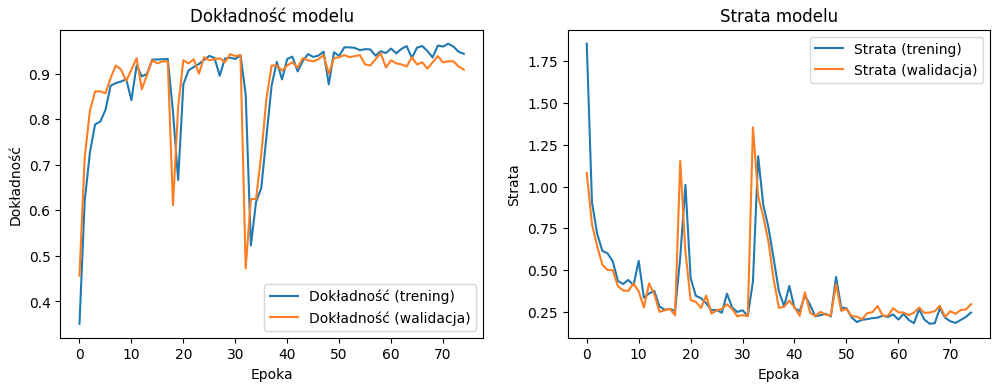
\includegraphics[width=15.5cm]{resources/tests/images/v3/base4_img.png}
	\caption{Wyniki testów dla modelu podstawowego, liczba wierzchołków n = 4}
	\label{Fig:tests-base-1a}
\end{figure}
\FloatBarrier

Ogólnie rzecz biorąc, model wydaje się dobrze uczyć na danych treningowych i~generalizować na danych walidacyjnych,
chociaż zmienność straty walidacyjnej może wskazywać na pewne problemy z~przeuczeniem.

\begin{figure}[ht]
	\centering
	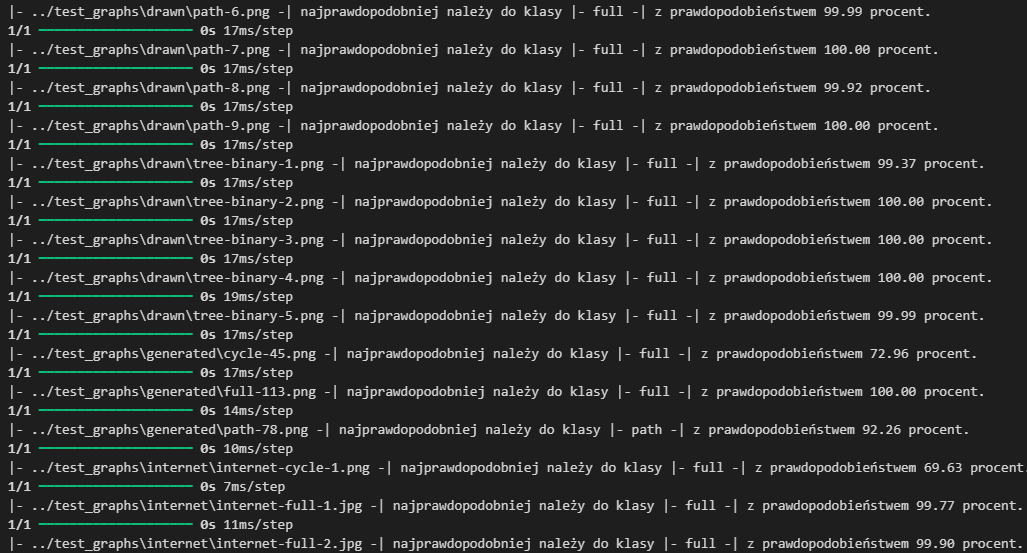
\includegraphics[width=15.5cm]{resources/tests/images/v3/base4_txt.png}
	\caption{Klasyfikacja obrazów zewnętrznych dla modelu podstawowego, liczba wierzchołków n = 4}
	\label{Fig:tests-base-1b}
\end{figure}
\FloatBarrier

\begin{figure}[ht]
	\centering
	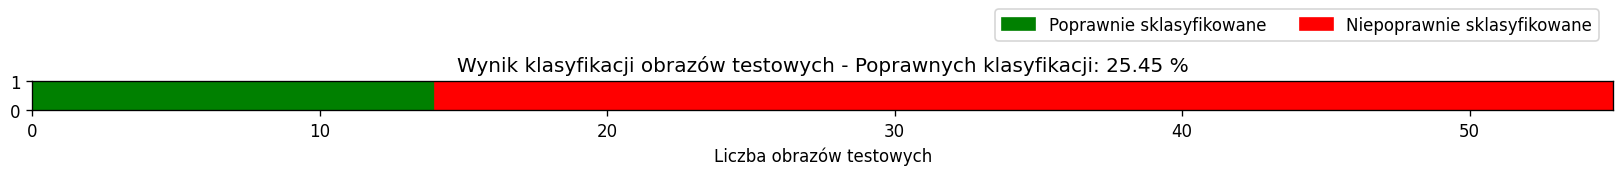
\includegraphics[width=15.5cm]{resources/tests/images/v3/base4_bar.png}
	\caption{Wizualizacja klasyfikacji obrazów zewnętrznych dla modelu podstawowego, liczba wierzchołków n = 4}
	\label{Fig:tests-base-1c}
\end{figure}
\FloatBarrier

Model przewidział poprawnie 25\% grafów, co nie jest najgorszym wynikiem,
zaważając że jest to najbardziej podstawowa wersja testowanego modelu.

\begin{figure}[ht]
	\centering
	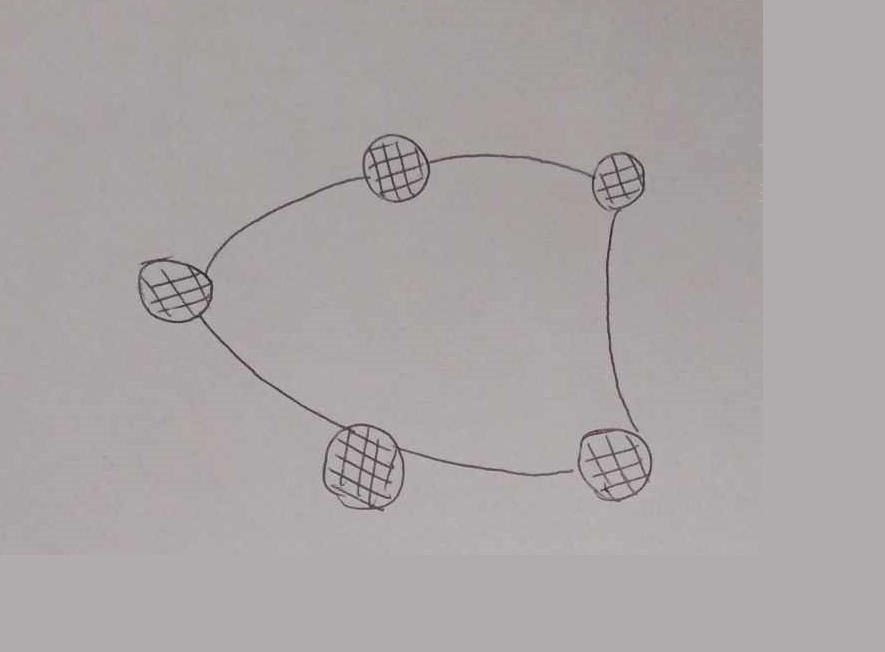
\includegraphics[height=4cm]{../graph_classification/test_graphs/drawn/cycle-1.png}
	\caption{Klasyfikacja przykładowego grafu zewnętrznego przez model podstawowy uczony na grafach czterowierzchołkowych.
		Przypisana klasa to graf pełny z~99,97\% pewnością.}
	\label{Fig:tests-base-1d}
\end{figure}
\FloatBarrier

% \begin{figure}[ht]
% 	\centering
% 	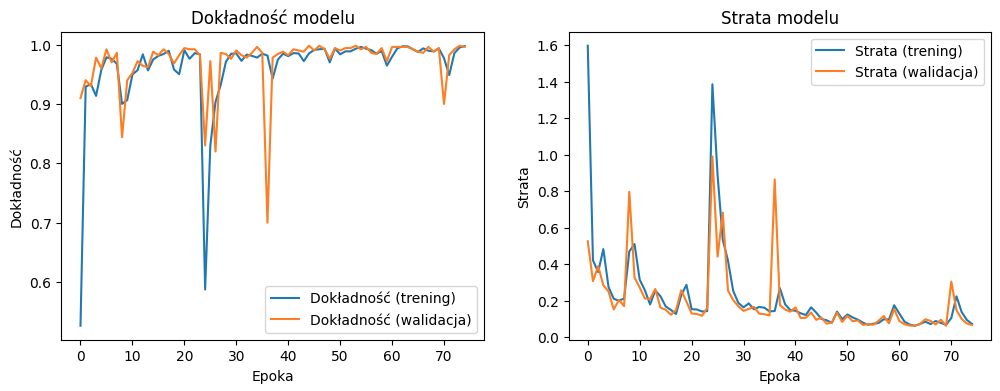
\includegraphics[width=15.5cm]{resources/tests/images/v3/base5_img.png}
% 	\caption{Wyniki testów dla modelu podstawowego, liczba wierzchołków n = 5}
% 	\label{Fig:tests-base-2a}
% \end{figure}
% \FloatBarrier

% \begin{figure}[ht]
% 	\centering
% 	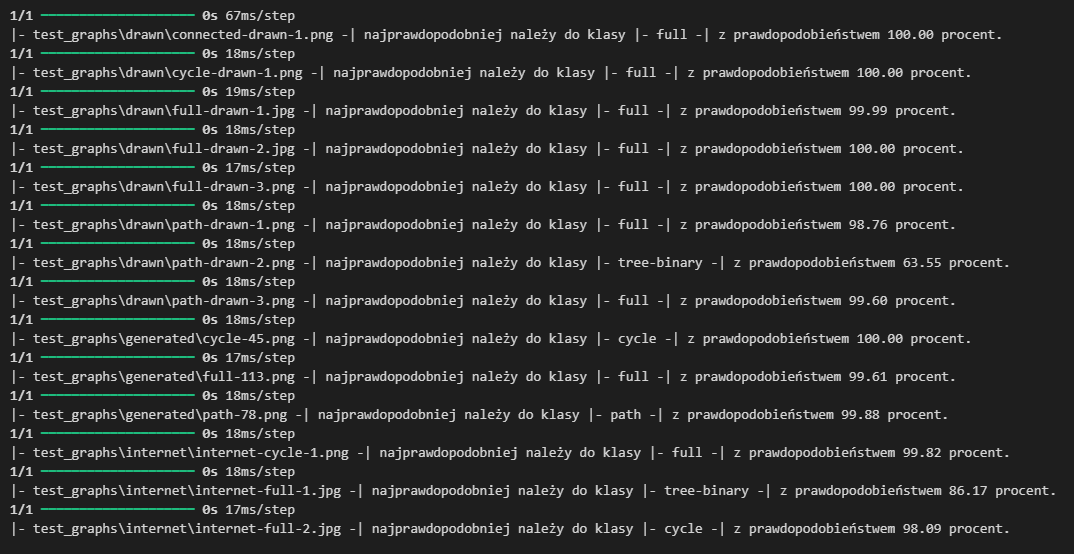
\includegraphics[width=15.5cm]{resources/tests/images/v3/base5_txt.png}
% 	\caption{Klasyfikacja obrazów zewnętrznych dla modelu podstawowego, liczba wierzchołków n = 5}
% 	\label{Fig:tests-base-2b}
% \end{figure}
% \FloatBarrier

% \begin{figure}[ht]
% 	\centering
% 	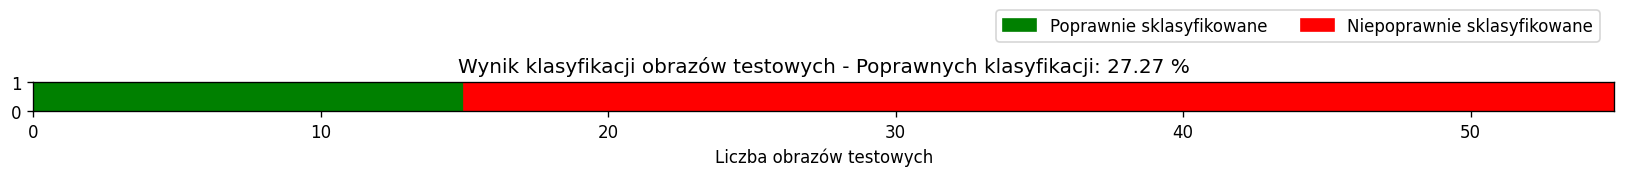
\includegraphics[width=15.5cm]{resources/tests/images/v3/base5_bar.png}
% 	\caption{Wizualizacja klasyfikacji obrazów zewnętrznych dla modelu podstawowego, liczba wierzchołków n = 5}
% 	\label{Fig:tests-base-2c}
% \end{figure}
% \FloatBarrier

\subsubsection{Model podstawowy uczony na grafach sześciowierzchołkowych}

Kolejny warty uwagi wynik został uzyskany za pomocą podstawowego modelu, ale uczonego na grafach o~sześciu wierzechołkach.
Dokładność zarówno dla zbioru treningowego, jak i~walidacyjnego, bardzo szybko wzrasta już w~kilku pierwszych epokach
i~osiąga bardzo wysoki wynik, bo prawie 100\%.
Występuje kilka spadków obu krzywych, z~czego jeden nawet do 80\%.
Ogólnie, po około 10 epokach, dokładność dla obu zestawów danych jest bardzo zbliżona i~stabilizuje się na poziomie około 99\%.

Strata, podobnie jak dokładność, spada w~ciągu początkowych epok procesu nauczania do niskich wartości, bo około 0,25.
W ciągu kolejnych epok, aż do końca, widać minimalny trend malejący, z~trzema wzrostami straty do około wartości 0,5 na zbiorze walidacyjnym.
Może to oznaczać, że w~tych punktach model napotyka na trudniejsze przypadki testowe.

\begin{figure}[ht]
	\centering
	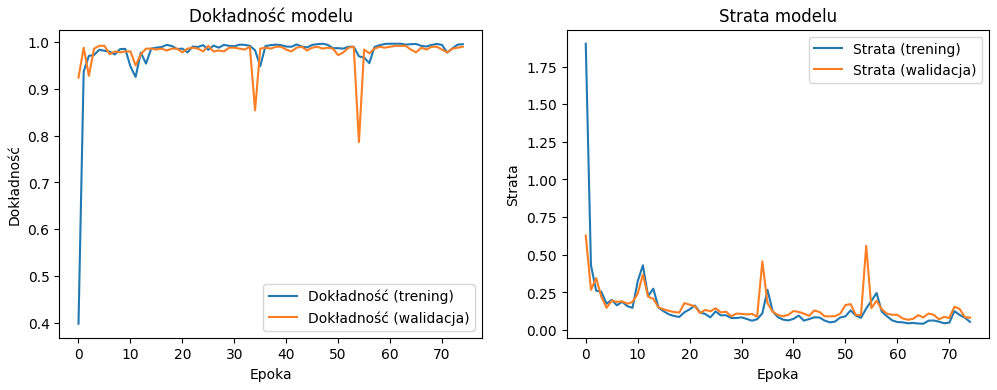
\includegraphics[width=15.5cm]{resources/tests/images/v3/base6_img.png}
	\caption{Wyniki testów dla modelu podstawowego, liczba wierzchołków n = 6}
	\label{Fig:tests-base-3a}
\end{figure}
\FloatBarrier

Różnice między wartościami straty i~dokładności dla zbioru walidacyjnego i~testowego są niewielkie.
Nie widać również znaczących fluktuacji.
Krzywe dokładności i~straty sugerują, że model może być poprawnie nauczony ogólnych wzorców
i~nie być nadmiernie dopasowanym do danych treningowych.

\begin{figure}[ht]
	\centering
	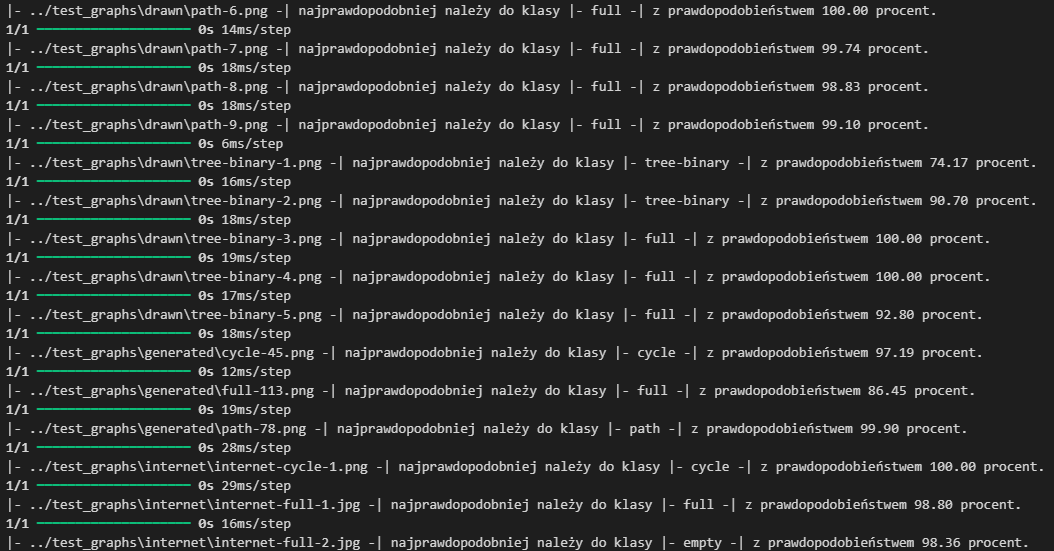
\includegraphics[width=15.5cm]{resources/tests/images/v3/base6_txt.png}
	\caption{Klasyfikacja obrazów zewnętrznych dla modelu podstawowego, liczba wierzchołków n = 6}
	\label{Fig:tests-base-3b}
\end{figure}
\FloatBarrier

\begin{figure}[ht]
	\centering
	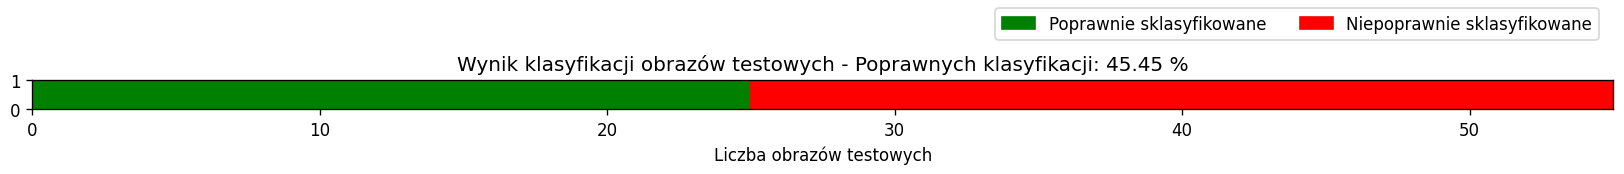
\includegraphics[width=15.5cm]{resources/tests/images/v3/base6_bar.png}
	\caption{Wizualizacja klasyfikacji obrazów zewnętrznych dla modelu podstawowego, liczba wierzchołków n = 6}
	\label{Fig:tests-base-3c}
\end{figure}
\FloatBarrier

Model poprawnie klasyfikuje ponad 45\% przypadków grafów zewnętrznych,
co jest zaskakująco wysokim wynikiem, zważając na niską złożoność owego modelu.
Czterdziestopięcioprocentowa dokładnośc przy klasyfikacji pięciu klas,
jest wynikiem zdecydowanie lepszym niż przypisywanie klas grafów losowo.

\begin{figure}[ht]
	\centering
	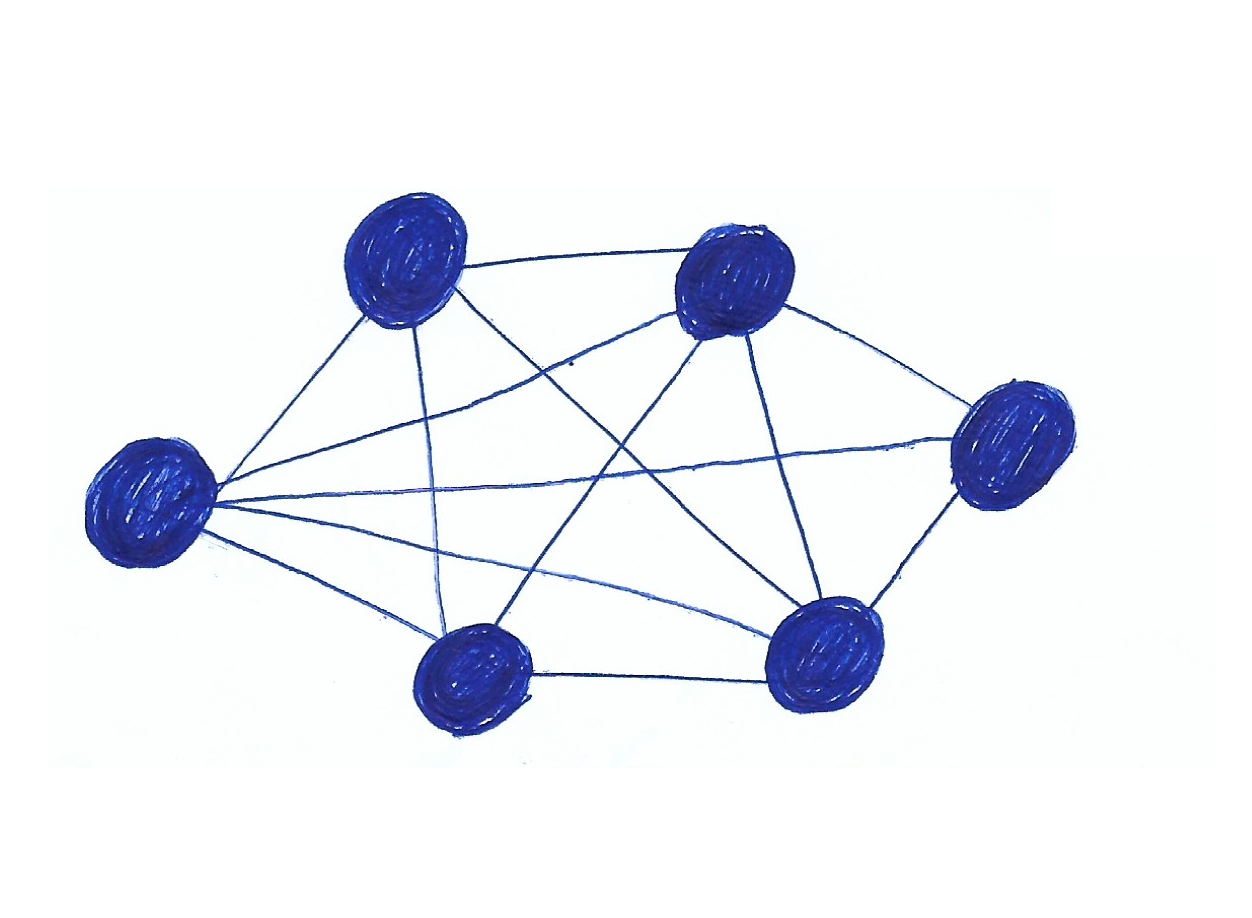
\includegraphics[height=4cm]{../graph_classification/test_graphs/drawn/full-9.png}
	\caption{Klasyfikacja przykładowego grafu zewnętrznego przez model podstawowy uczony na grafach sześciowierzchołkowych.
		Przypisana klasa to graf pełny z~100\% pewnością.}
	\label{Fig:tests-base-3d}
\end{figure}
\FloatBarrier

% \begin{figure}[ht]
% 	\centering
% 	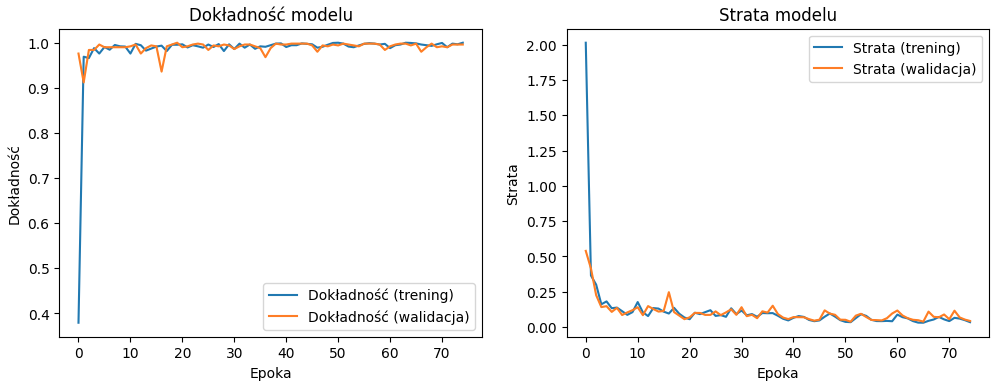
\includegraphics[width=15.5cm]{resources/tests/images/v3/base7_img.png}
% 	\caption{Wyniki testów dla modelu podstawowego, liczba wierzchołków n = 7}
% 	\label{Fig:tests-base-4a}
% \end{figure}
% \FloatBarrier

% \begin{figure}[ht]
% 	\centering
% 	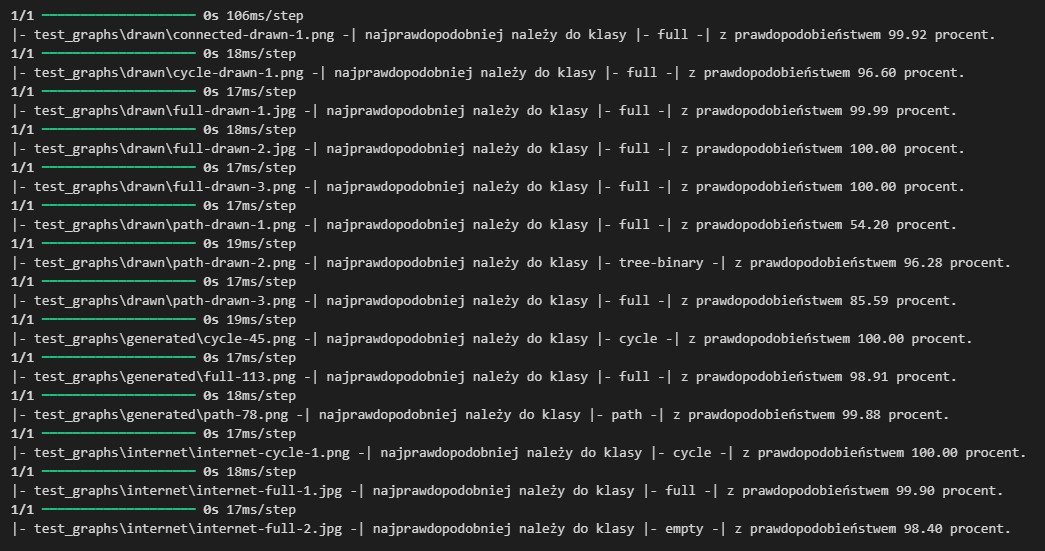
\includegraphics[width=15.5cm]{resources/tests/images/v3/base7_txt.png}
% 	\caption{Klasyfikacja obrazów zewnętrznych dla modelu podstawowego, liczba wierzchołków n = 7}
% 	\label{Fig:tests-base-4b}
% \end{figure}
% \FloatBarrier

% \begin{figure}[ht]
% 	\centering
% 	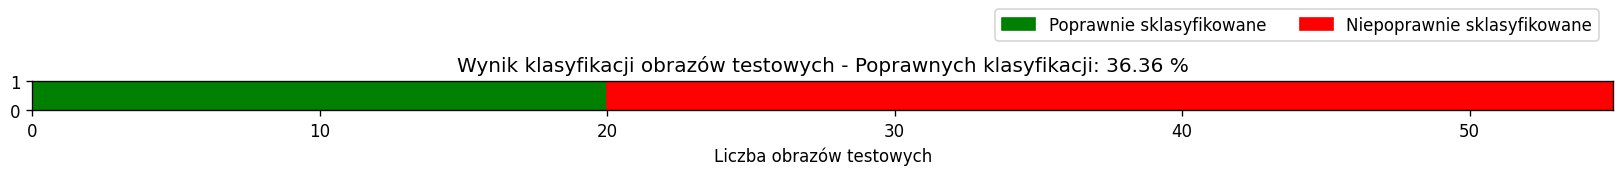
\includegraphics[width=15.5cm]{resources/tests/images/v3/base7_bar.png}
% 	\caption{Wizualizacja klasyfikacji obrazów zewnętrznych dla modelu podstawowego, liczba wierzchołków n = 7}
% 	\label{Fig:tests-base-4c}
% \end{figure}
% \FloatBarrier

\section{Model z~walidacją krzyżową}
% \textbf{Model uczony na stałej krzywiźnie wierzechołków}

% \begin{figure}[ht]
% 	\centering
% 	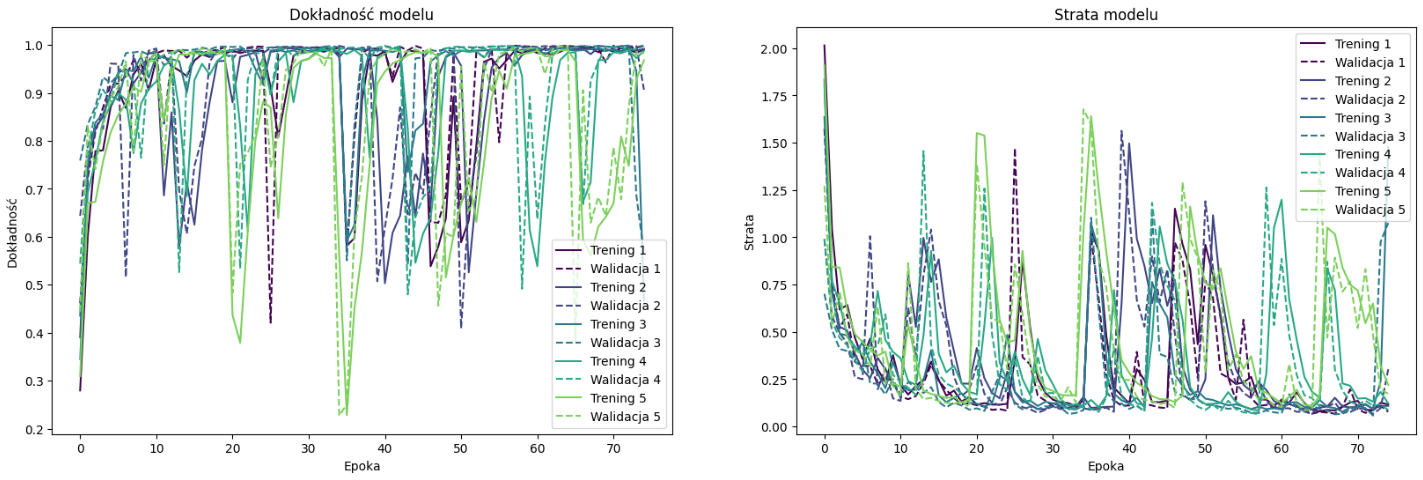
\includegraphics[height=5.5cm]{resources/tests/images/v2/crossvalid_img.png}
% 	\caption{Wyniki testów dla modelu z walidacją krzyżową i stałą krzywizną wierzechołków}
% 	\label{Fig:tests-cv-1}
% \end{figure}
% \FloatBarrier

% \begin{figure}[ht]
% 	\centering
% 	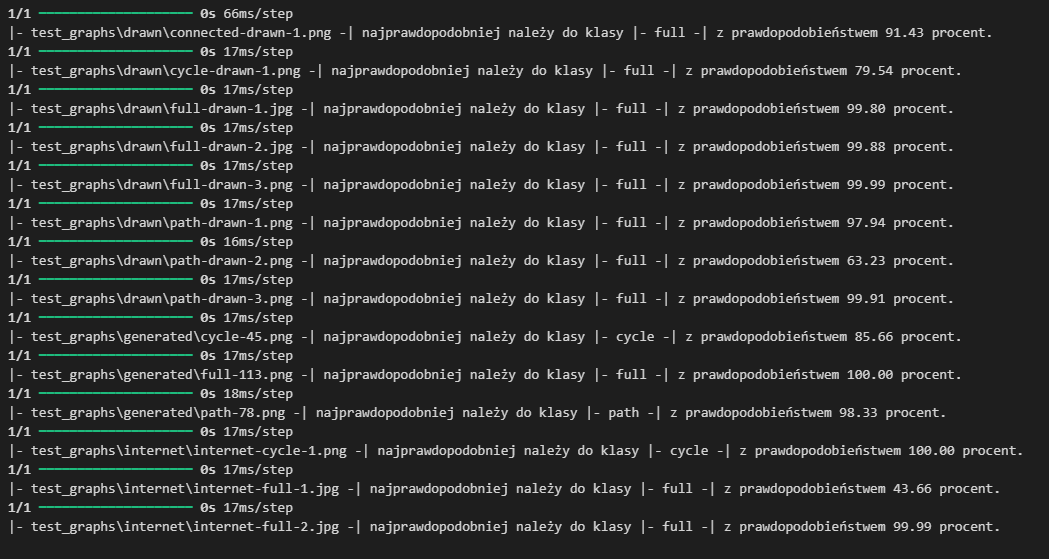
\includegraphics[height=7cm]{resources/tests/images/v2/crossvalid_txt.png}
% 	\caption{Klasyfikacja obrazów zewnętrznych dla modelu z walidacją krzyżową i stałą krzywizną wierzechołków}
% 	\label{Fig:tests-cv-2}
% \end{figure}
% \FloatBarrier

\textbf{Model uczony na losowej krzywiźnie wierzechołków}

W przypadku modelu z walidacją krzyżową, uczonego na grafach z 4 wierzchołkami,
dokładność wzrasta gwałtownie na początku treningu,
osiągając wartości powyżej 0.8 już po około 10 epokach.
Dokładność stabiliziuje się w okolicach 90\%, ale mimo to widać pewne fluktuacje, zwłaszacza na danych walidacyjnych.
Możliwe do zaobserowania są regularne spadki dokładności w niektórych epokach,
co może wynikać z niestabilnego treningu lub problemów modelu w generalizacji dla niektórych danych walidacyjncyh.

Dla straty modelu można zaobserować spadek w pierwszych 10 epokach, co mogłoby wskazywać na szybkie uczenie się modelu.
Zaraz po nim, następuje stabilizacja na niskim poziomie, z pojedynczymi skokami, głównie na zbiorze walidacyjnym.
Nieregularne wzrosty straty, podobnie jak w przypadku dokładności, mogą wskazywać na problemy z przeuczeniem.

\begin{figure}[ht]
	\centering
	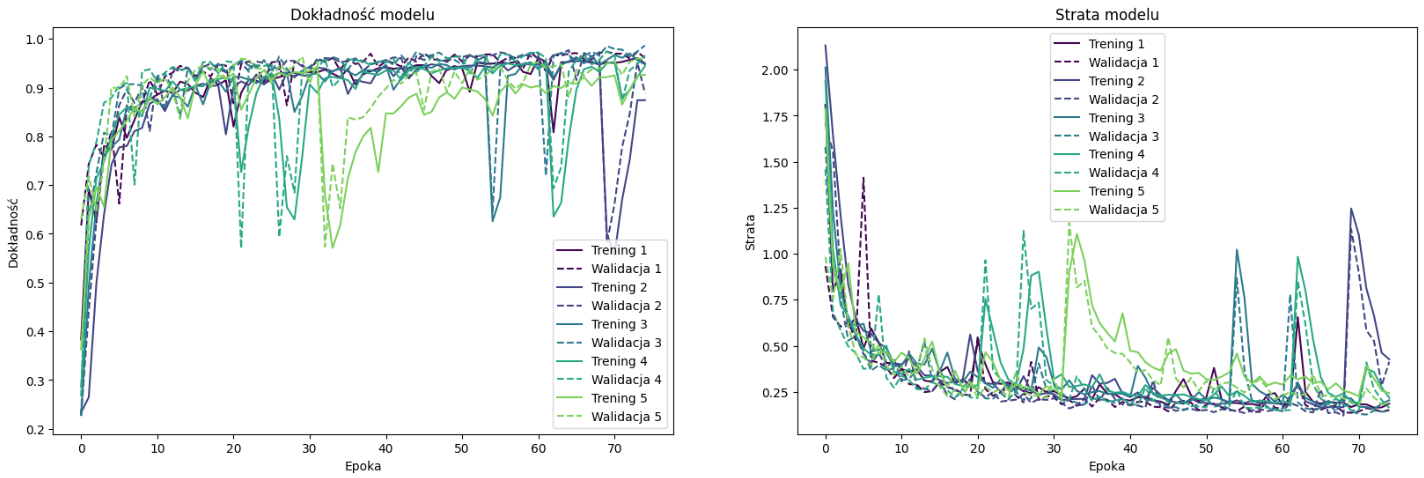
\includegraphics[height=5.5cm]{resources/tests/images/v3/crossvalid_img.png}
	\caption{Wyniki testów dla modelu z walidacją krzyżową i losową krzywizną wierzchołków}
	\label{Fig:tests-cv-1}
\end{figure}
\FloatBarrier

Podsumowując, ten wariant modelu generalnie uczy się poprawnie, dzięki czemu osiąga wysoką dokładność i niską stratę.
Fluktuacje jakie występują w wynikach, szczególnie na danych walidacyjnych,
sugerują jednak potencjalne problemy z generalizacją, co może być wynikiem niestabilności modelu,
przeuczenia modelu, lub trudności w rozpoznawaniu bardziej złożonych przykładów w danych walidacyjnych.

W przypadku tego modelu, zwiększenie liczby epok, nie przyniosłoby zamierzonych skutków.
Model zbyt szybko się przeucza, a więc większa liczba iteracji nie wpłynęłaby w żaden znaczący sposób na wynik.

\begin{figure}[ht]
	\centering
	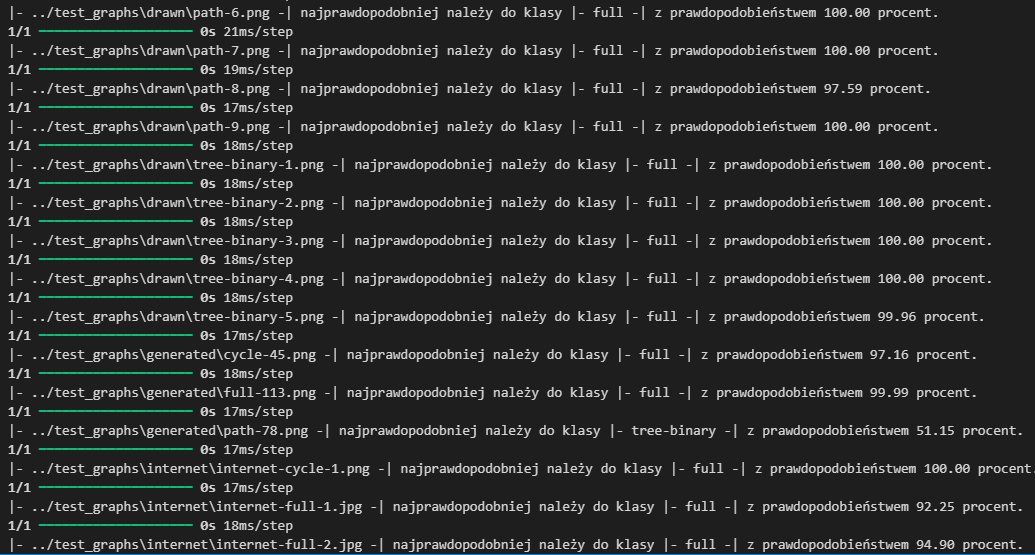
\includegraphics[height=7cm]{resources/tests/images/v3/crossvalid_txt.png}
	\caption{Klasyfikacja obrazów zewnętrznych dla modelu z walidacją krzyżową i losową krzywizną wierzchołków}
	\label{Fig:tests-cv-2}
\end{figure}
\FloatBarrier

Z powodu przeuczenia model nie radził sobie z zewnętrznymi obrazkami testowymi.
Większość grafów określił jako grafy pełne, a jedną ze scieżek jako drzewo binarne,
co nie jest zgodne ze stanem rzeczywistym.

\textbf{Zmodyfikowany model}

W celu poprawy dokładności i zapobiegnięciu przeuczenia wprowadzone
zostały następujące modyfikacje do modelu z walidacją krzyżową.
Każde z nich zostało przetestowane w osobnym modelu.
Stworzony został również jeden model ze wszystkimi połączonymi modyfikacjami. 
\begin{itemize}[label=-,labelsep=0.4cm,leftmargin=0.6cm]
    \item Zmieniono liczbę filtrów w warstwach Conv2D z 32 w każdej warstwie, do kolejno 32, 64 oraz 128.
		Jednocześnie zwiększono parametr Dropout z 0,2 do 0,5.
    \item Zastosowano Batch Normalization pomiędzy warstwami modelu - konkretnie po każdej warstwie Conv2D.
    \item Wprowadzenie augmentacji danych przed budową modelu, która wprowadza więcej wariacji do zbioru treningowego,
		w celu poprawy zdolności generalizacyjnych.
		Wykorzystano również GPU w procesie prefetchingu i cachingu zbiorów danych, by przypsieszyć przetwarzanie danych.
	\item Skorzystanie z wywołania zwrotnego, które zmniejsza szybkość uczenia.
		W przypadku stagnacji dokładności w procesie przechodzenia przez kolejne epoki uczenia modelu
		może pomóc w lepszej konwergencji modelu.
\end{itemize}

\textbf{Zmodyfikowany model - Conv2D i Dropout}

Wszystkie przebiegi walidacji krzyżowej osiągają wysoką dokładność po kilku pierwszych epokach.
Model bardzo szybko uczy się rozpoznawać wzorce.
Walidacja również osiąga zadoalające wyniki, tj. około 90\%. Może to wskazywać na poprawną generalizację do nowych danych.
Występuje jednak niewielka niesabilność, występująca pomiędzy epokami,
co widać po gwałtownych spadkach i wzrostach dokładności walidacji.

Strata na zbiorze treningowym i walidacyjnym systematycznie maleje z kolejnymi epokami,
co może wskazywać na dobre dopasowanie do danych treningowych.
Zauważalnym problemem jest jednak spora fluktuacja obu wskaźników.
Model może napotykać trudności z pewnymi próbkami w zbiorze danych walidacyjnych. 

\begin{figure}[ht]
	\centering
	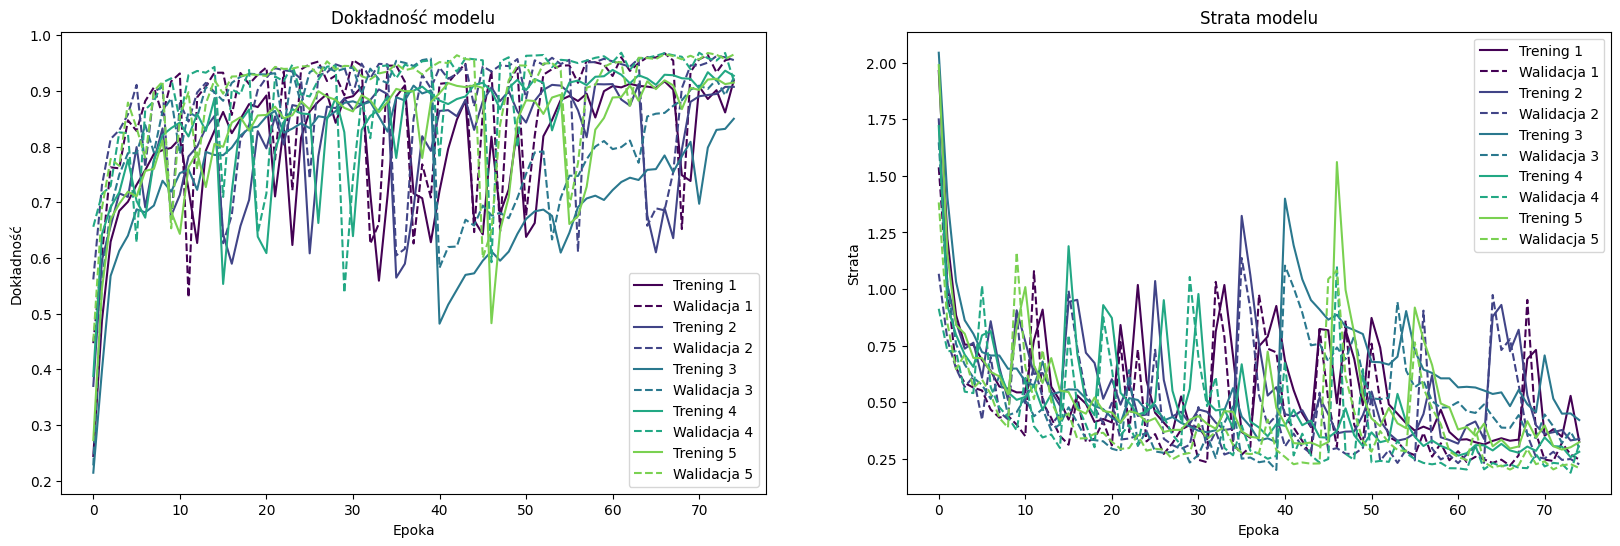
\includegraphics[height=5.5cm]{resources/tests/images/v4/crossvalid_1_img.png}
	\caption{Wyniki testów dla zmodyfikowanego modelu z walidacją krzyżową i losową krzywizną wierzchołków}
	\label{Fig:tests-cv-1}
\end{figure}
\FloatBarrier

Modfyikacja modelu wydaje się osiągać zamierzone skutki,
ponieważ model wykazuje lepszą zdolność uczenia z danych treningowych
oraz osiąga wysoką dokładność na danych walidacyjnych.
Model może być jednak wrażliwy na trudniejsze przypadki ze zbioru danych walidacyjnych,
zważając na wahania wskaźników.

\begin{figure}[ht]
	\centering
	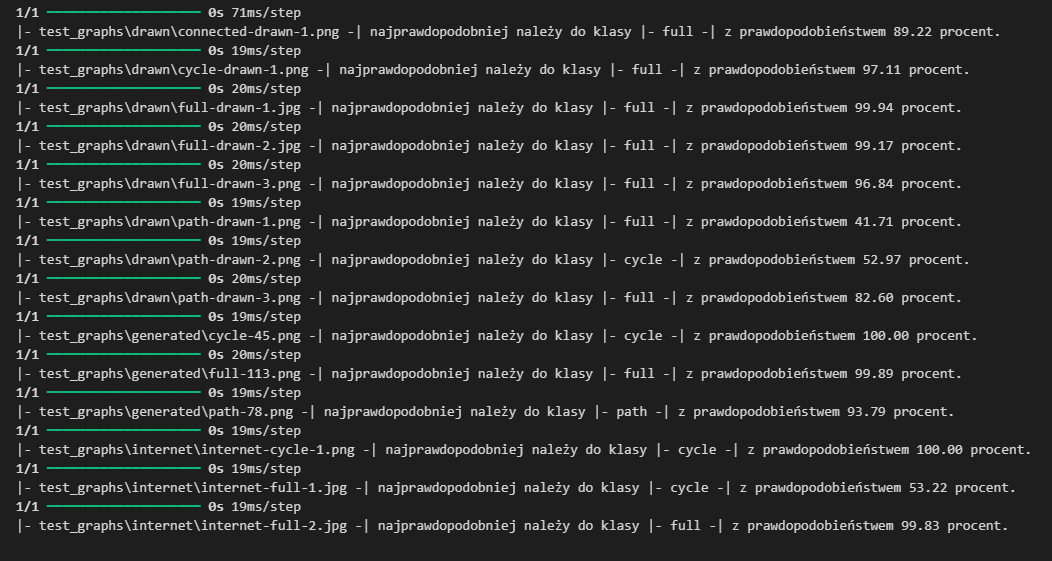
\includegraphics[height=5.5cm]{resources/tests/images/v4/crossvalid_1_txt.png}
	\caption{Wyniki testów dla zmodyfikowanego modelu z walidacją krzyżową i losową krzywizną wierzchołków}
	\label{Fig:tests-cv-1}
\end{figure}
\FloatBarrier

Model poprawnie sklasyfikował 9 rysunków grafów,
co jest znacznym polepszeniem w stosunku do początkowego modelu z zastosowaną walidacją krzyżową.

\textbf{Zmodyfikowany model - Batch Normalization}

Model został zmodyfikowany poprzez zastosowanie batch normalization pomiędzy kolejnymi warstwami Conv2D modelu.
Ma to na celu poprawienie stabilności treningu oraz przyspieszenie uczenia.
Użyte zostało również zwiększenie liczby filtrów w warstwach Conv2D oraz zwiększenie parametru Dropout
z poprzedniej modyfikacji modelu, ponieważ osięgnęła ona zamierzone cele.

\begin{lstlisting}[language=Python,caption=Listing zmodyfikowanego skryptu tworzącego model z walidacją krzyżową,
	label={tests-model-crossval2}]
	model = tf.keras.models.Sequential([
      tf.keras.layers.Rescaling(1./255),
      tf.keras.layers.Conv2D(32, 3, activation='relu'),
      tf.keras.layers.BatchNormalization(),
      tf.keras.layers.MaxPooling2D(),
      tf.keras.layers.Conv2D(64, 3, activation='relu'),
      tf.keras.layers.BatchNormalization(),
      tf.keras.layers.MaxPooling2D(),
      tf.keras.layers.Conv2D(128, 3, activation='relu'),
      tf.keras.layers.BatchNormalization(),
      tf.keras.layers.MaxPooling2D(),
      tf.keras.layers.Flatten(),
      tf.keras.layers.Dense(128, activation='relu', kernel_regularizer=tf.keras.regularizers.l2(0.01)),
      tf.keras.layers.Dropout(0.5),
      tf.keras.layers.Dense(len(class_names))
  ])
\end{lstlisting}

Na wykresach dokładności treningowych widać stały wzrost od około 70\% do prawie 100\%.
Jest to oczywiście pozytywna cecha modelu, lecz po analizie krzywych dokładności walidacyjnych,
należy stwierdzić, że jest to przeuczenie. Model poprawnie nauczył się danych treningowych,
lecz nie zapamiętał ogólnych wzorców, zważając na wysokie wahania oraz niestałość walidacji.

Strata treningowa, co jest spodziewane po uznaniu model za przeuczony,
osiąga bardzo niskie wartości treingowe - przez wszystkie epoki jest bliska 0.
Strata walidacyjna zaś, mimo że pozornie wygląda na stabilną, taka nie jest
- należy zwrócić uwagę na jednostki na skali. Wahania są bardzo duże oraz występuje pojedyncza wartość odstająca,
która osiąga ponad 6000 jednostek.

\begin{figure}[ht]
	\centering
	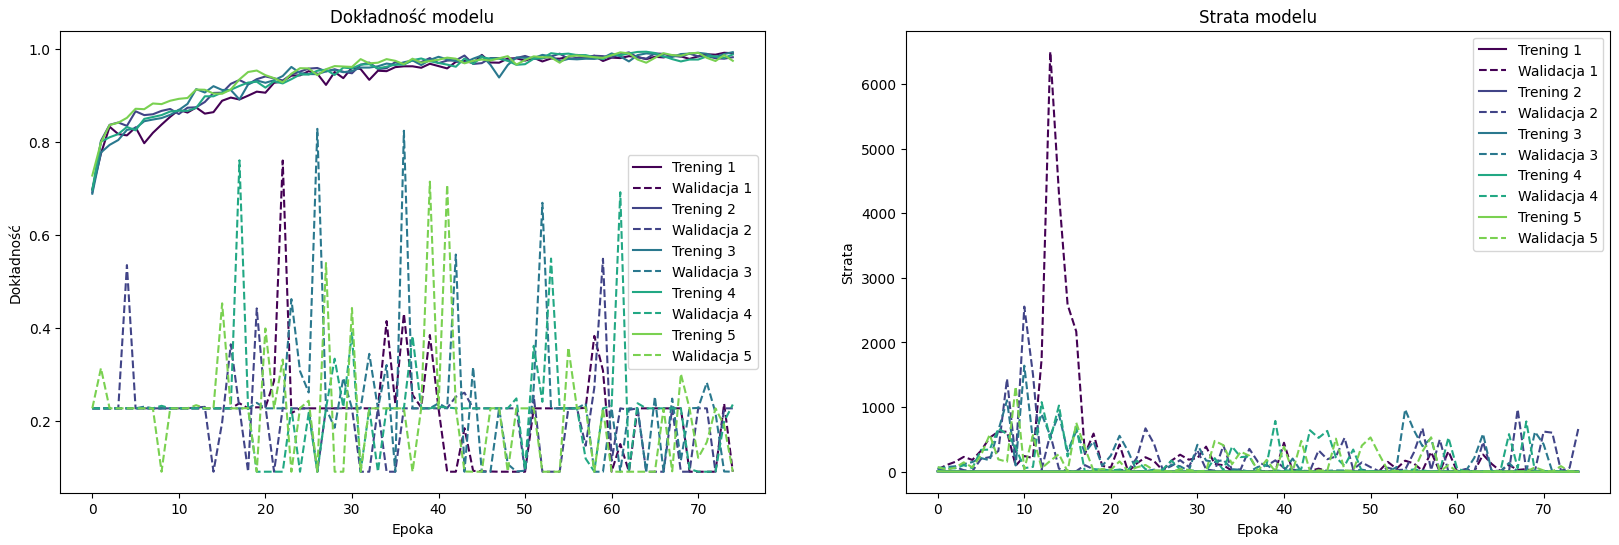
\includegraphics[height=5.5cm]{resources/tests/images/v4/crossvalid_2_img.png}
	\caption{Wyniki testów dla zmodyfikowanego modelu z walidacją krzyżową i losową krzywizną wierzchołków}
	\label{Fig:tests-cv-1}
\end{figure}
\FloatBarrier

Ogólne % ------ TO DO ------ %

\begin{figure}[ht]
	\centering
	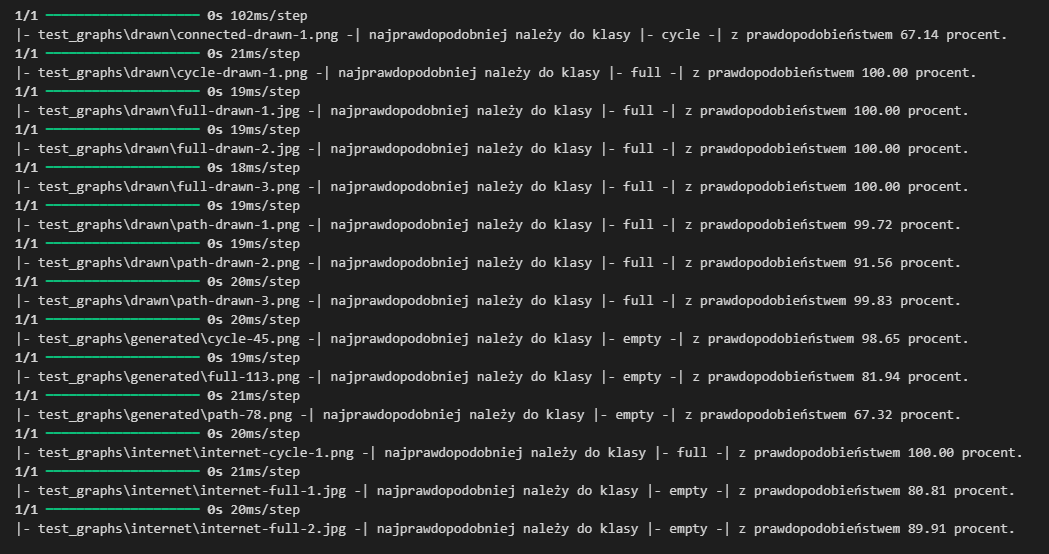
\includegraphics[height=5.5cm]{resources/tests/images/v4/crossvalid_2_txt.png}
	\caption{Wyniki testów dla zmodyfikowanego modelu z walidacją krzyżową i losową krzywizną wierzchołków}
	\label{Fig:tests-cv-1}
\end{figure}
\FloatBarrier

Opis klasyfikacji % ------ TO DO ------ %

\textbf{Zmodyfikowany model - Augmentacja danych}

Opis modyfikacji % ------ TO DO ------ %

Dokładność % ------ TO DO ------ %

Strata % ------ TO DO ------ %

\begin{figure}[ht]
	\centering
	% 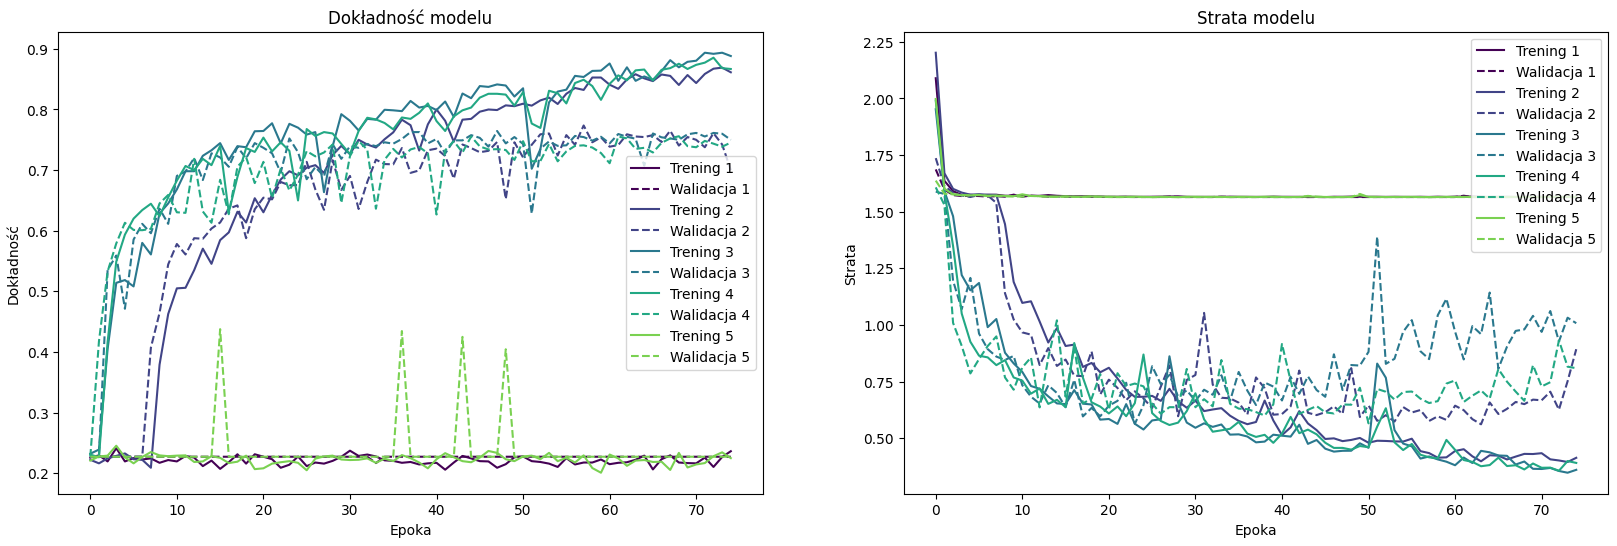
\includegraphics[height=5.5cm]{resources/tests/images/v4/crossvalid_3_img.png}
	\caption{Wyniki testów dla zmodyfikowanego modelu z walidacją krzyżową i losową krzywizną wierzchołków}
	\label{Fig:tests-cv-1}
\end{figure}
\FloatBarrier
Ogólne % ------ TO DO ------ %

\begin{figure}[ht]
	\centering
	% 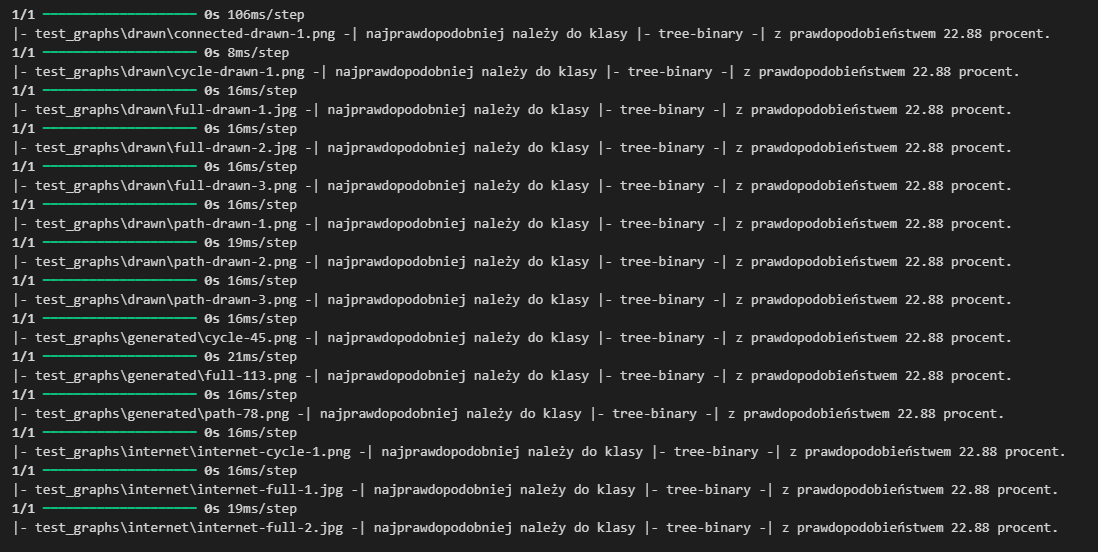
\includegraphics[height=5.5cm]{resources/tests/images/v4/crossvalid_3_txt.png}
	\caption{Wyniki testów dla zmodyfikowanego modelu z walidacją krzyżową i losową krzywizną wierzchołków}
	\label{Fig:tests-cv-1}
\end{figure}
\FloatBarrier

Opis klasyfikacji % ------ TO DO ------ %

\textbf{Zmodyfikowany model - Spowolnienie uczenia}

Opis modyfikacji % ------ TO DO ------ %

Dokładność % ------ TO DO ------ %

Strata % ------ TO DO ------ %

\begin{figure}[ht]
	\centering
	% 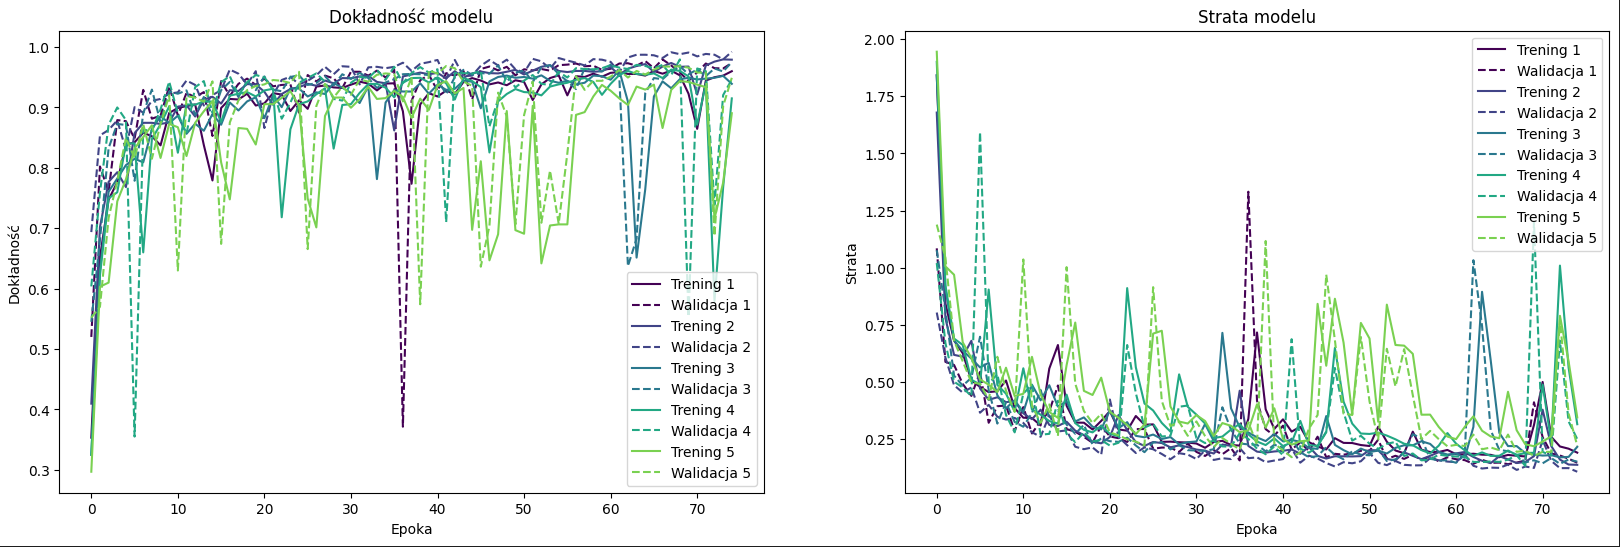
\includegraphics[height=5.5cm]{resources/tests/images/v4/crossvalid_4_img.png}
	\caption{Wyniki testów dla zmodyfikowanego modelu z walidacją krzyżową i losową krzywizną wierzchołków}
	\label{Fig:tests-cv-1}
\end{figure}
\FloatBarrier

Ogólne % ------ TO DO ------ %

\begin{figure}[ht]
	\centering
	% 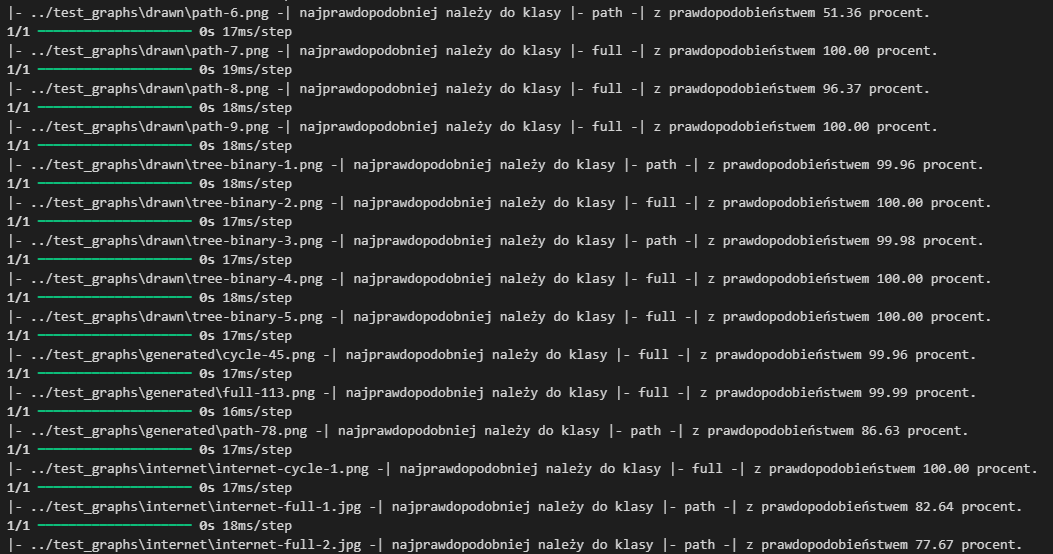
\includegraphics[height=5.5cm]{resources/tests/images/v4/crossvalid_4_txt.png}
	\caption{Wyniki testów dla zmodyfikowanego modelu z walidacją krzyżową i losową krzywizną wierzchołków}
	\label{Fig:tests-cv-1}
\end{figure}
\FloatBarrier

Opis klasyfikacji % ------ TO DO ------ %

\textbf{Zmodyfikowany model połączony}

Dokładność dla wszystkich przebiegów stopniowo wzrasta wraz z liczbą epok
i osiąga wysoki poziom, bo powyżej 80\%, pod koniec treningu.
W przypadku walidacji jednak, wyniki nie są zadowalające, a wrecz bardzo niestabilne.
Przez większość przebiegów uczenia utrzymuje się na niskim poziomie,
co może sugerować problemy z generalizacją danych.

Strata treningowa maleje w większości przebiegów, co jest spodziewane podczas uczenia.
Widać jednak pewne fluktuacje, świadczące o problemach z konwergencją.
Dla straty walidacyjnej można zaobserować wielką niestabilność - osiąga bardzo wysokie wartości,
nawet rzędu kilku tysięcy, jak również bardzo niskie, bliskie zeru.

\begin{figure}[ht]
	\centering
	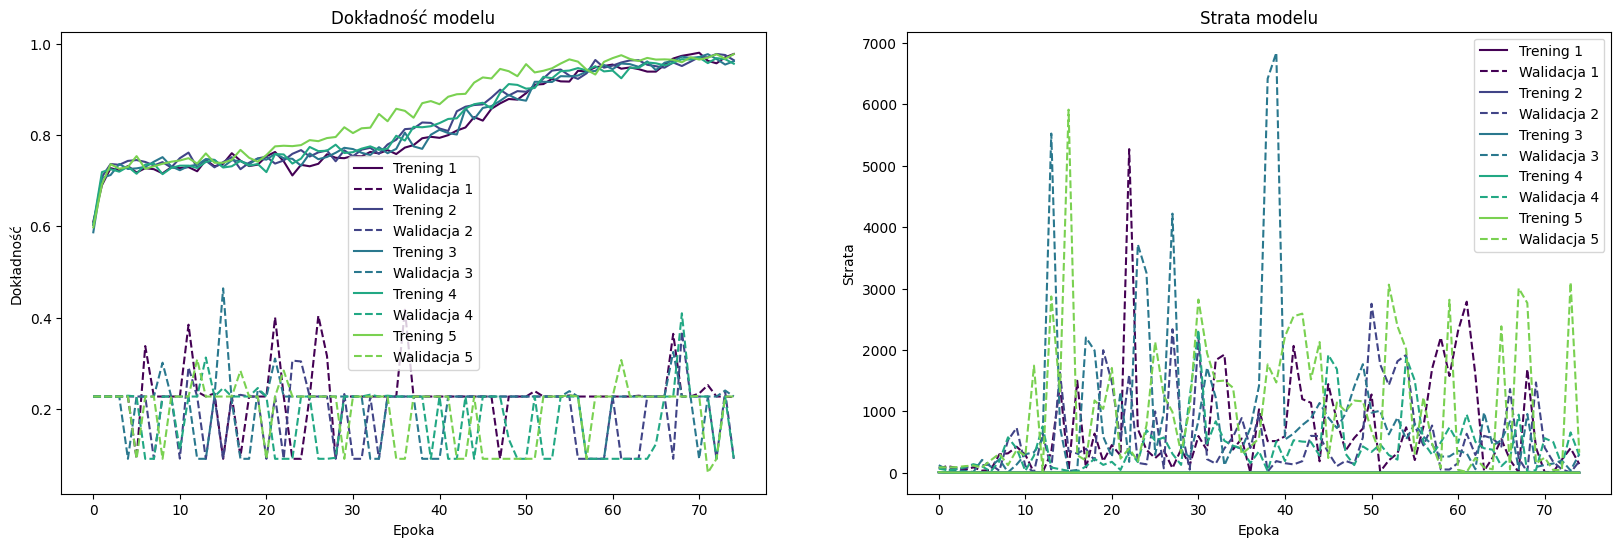
\includegraphics[height=5.5cm]{resources/tests/images/v4/crossvalid_img.png}
	\caption{Wyniki testów dla zmodyfikowanego modelu z walidacją krzyżową i losową krzywizną wierzchołków}
	\label{Fig:tests-cv-1}
\end{figure}
\FloatBarrier

Ogólne wnioski jakie można wyciągnąć z procesu uczenia tego modelu,
są takie, że model kompletnie nie radzi sobie z danymi walidacyjnymi.
Model ewidentnie przeucza się na danych treningowych,
podczas gdy jego wydajność na zbiorze walidacyjnym jest bardzo słaba.
Zastosowanie wszystkich zaproponowanych technik na raz,
nie osiągnęło zamierzonego skutku. 

\begin{figure}[ht]
	\centering
	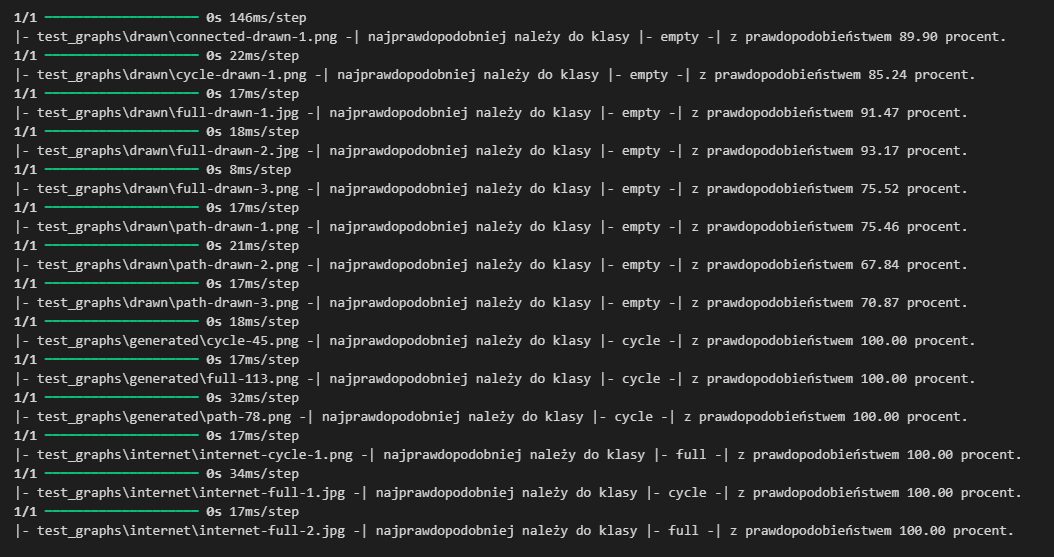
\includegraphics[height=7cm]{resources/tests/images/v4/crossvalid_txt.png}
	\caption{Klasyfikacja obrazów zewnętrznych dla zmodyfikowanego modelu z walidacją krzyżową i losową krzywizną wierzchołków}
	\label{Fig:tests-cv-2}
\end{figure}
\FloatBarrier

Model poprawnie wskazał klasy tylko dwóch grafów testowych, co jest znacznie poniżej oczekiwanych rezultatów.

\section{Model ze zmienną liczbą wierzchołków}
% \textbf{Model uczony na stałej krzywiźnie wierzechołków}

% \begin{figure}[ht]
% 	\centering
% 	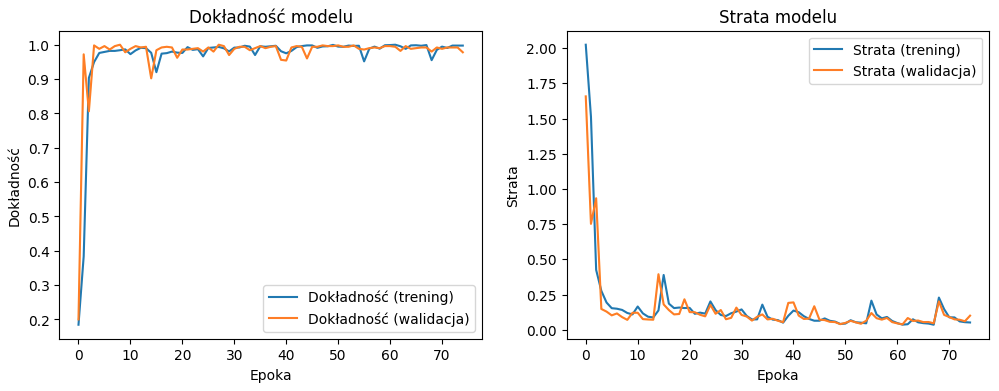
\includegraphics[height=5.5cm]{resources/tests/images/v2/multiple_edges_img.png}
% 	\caption{Wyniki testów dla modelu ze zmienną liczbą wierzchołków i stałą krzywizną wierzechołków}
% 	\label{Fig:tests-var-1}
% \end{figure}
% \FloatBarrier

% \begin{figure}[ht]
% 	\centering
% 	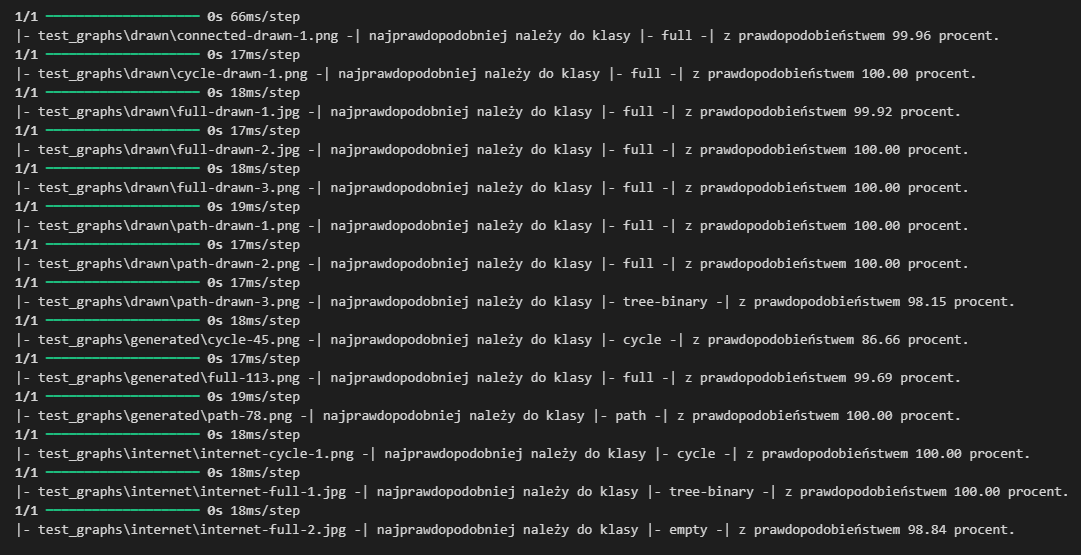
\includegraphics[width=14cm]{resources/tests/images/v2/multiple_edges_txt.png}
% 	\caption{Klasyfikacja obrazów zewnętrznych dla modelu z walidacją krzyżową i stałą krzywizną wierzechołków}
% 	\label{Fig:tests-var-2}
% \end{figure}
% \FloatBarrier

\textbf{Model uczony na losowej krzywiźnie wierzechołków} %--to do delet --%

Dokładność modelu uczonego na grafach treningowych z liczbą wierzchołków od czterech do siedmiu,
prezentuje się dość stabilnie po początkowej fazie wzrostu. Występują tylko drobne fluktuacje.
Po kilku początkowych epokach, dokładność oscyluje wokół 95\%, dochodząc nawet do 100\%.
Linie walidacji i treningu są bardzo blisko siebie, co sugeruje dobrą generalizację modelu
i nie wskazuje na przeuczenie.

W przypadku straty modelu, początkowy gwałtowny spadek sugeruje, że model dość szybko się uczy.
Po 10 epokach następuje stabilizacja straty na niskim, bo wynoszącym około 0.1, poziomie.
Podobnie jak w przypadku dokładności, strata dla zbioru walidacyjnego jest blisko straty treningowej.
Można zaobserować pewne wzrosty, które mogą być spowodowane trudniejszymi przypadkami w zbiorze walidacyjnym.

\begin{figure}[ht]
	\centering
	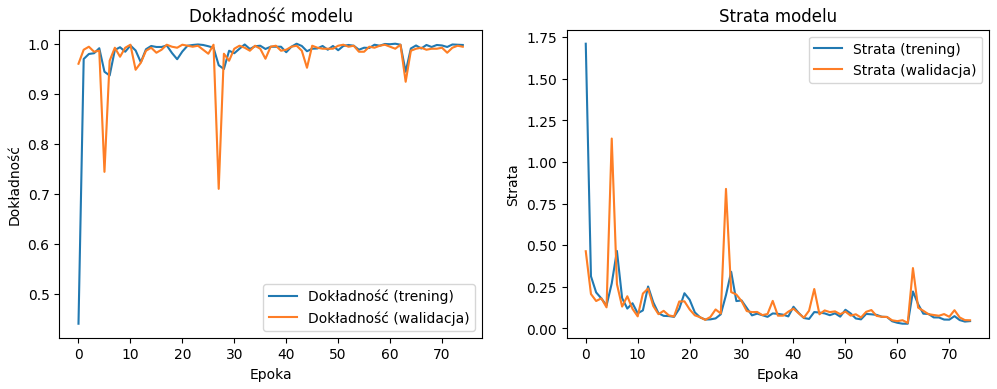
\includegraphics[height=5.5cm]{resources/tests/images/v3/multiple_edges_img.png}
	\caption{Dokładność i walidacja dla modelu ze zmienną liczbą wierzchołków}
	\label{Fig:tests-var-0a}
\end{figure}
\FloatBarrier

Model ten wydaje się być dobrze dopasywany i stabilny oraz poprawnie generalizujący.
Z uwagi na bliskość wyników dla treningu i walidacji, można stwierdzić, że model nie jest przeuczony.

\begin{figure}[ht]
	\centering
	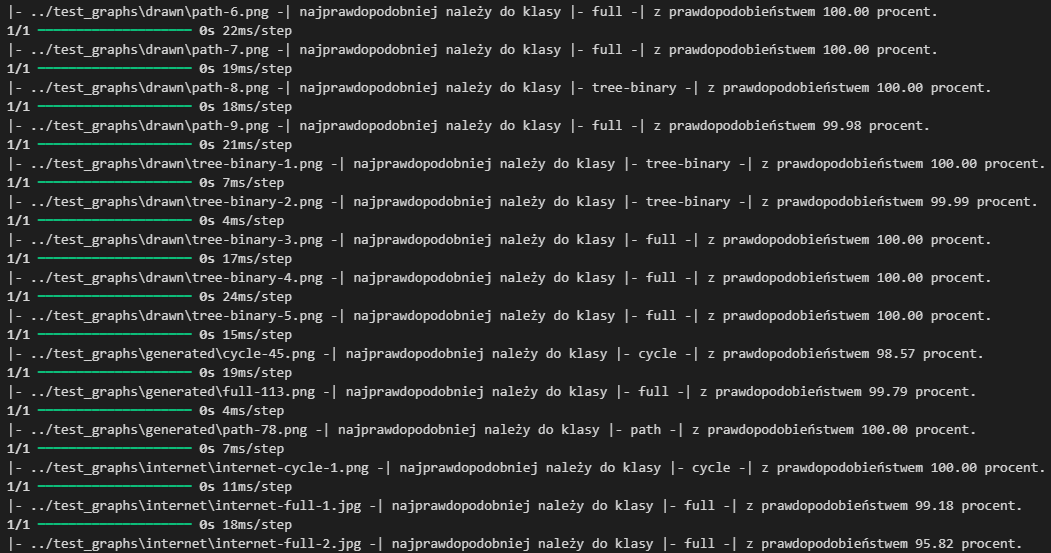
\includegraphics[width=14cm]{resources/tests/images/v3/multiple_edges_txt.png}
	\caption{Klasyfikacja obrazów zewnętrznych dla modelu ze zmienną liczbą wierzchołków}
	\label{Fig:tests-var-0b}
\end{figure}
\FloatBarrier

\begin{figure}[ht]
	\centering
	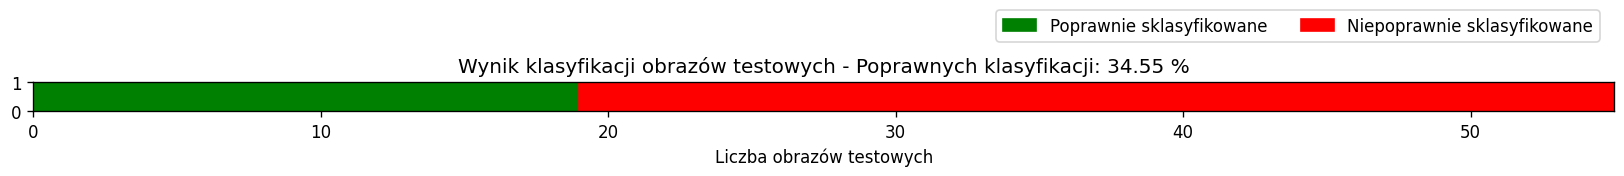
\includegraphics[width=14cm]{resources/tests/images/v3/multiple_edges_bar.png}
	\caption{Wizualizacja klasyfikacji obrazów zewnętrznych dla modelu ze zmienną liczbą wierzchołków}
	\label{Fig:tests-var-0c}
\end{figure}
\FloatBarrier

Model poprawnie sklasyfikował ponad 34\% rysunków zewnętrznych.
Nie jest to zły wynik, biorąc pod uwagę niską złożoność modelu.

\textbf{Zmodyfikowany model - Conv2D i Droput oraz spowolnienie uczenia}

W modelu wprowadzone zostało zwiększenie liczby filtrów dla warstw Conv2D, zwiększenie parametru Dropout
oraz zastosowano wywołanie zwrotne, które spowalnia uczenie.

Dokładność treningowa i walidacyjna modelu bardzo szybko wzrasta do wartości bliskich 100\%
i stabilizuje się na takim poziomie do końca procesu nauki.
Gdyby tylko dokładność treningowa osiągała taki poziom, możnaby założyć z dużą dozą pewności, przeuczenie modelu.
W tym przypadku jednak, różnice między dokładnością walidacyjną a treningową są marginalne.

Straty modelu wykazują podobne cechy do dokładności - szybki spadek wartości oraz stabilizacja na niskim poziomie.

\begin{figure}[ht]
	\centering
	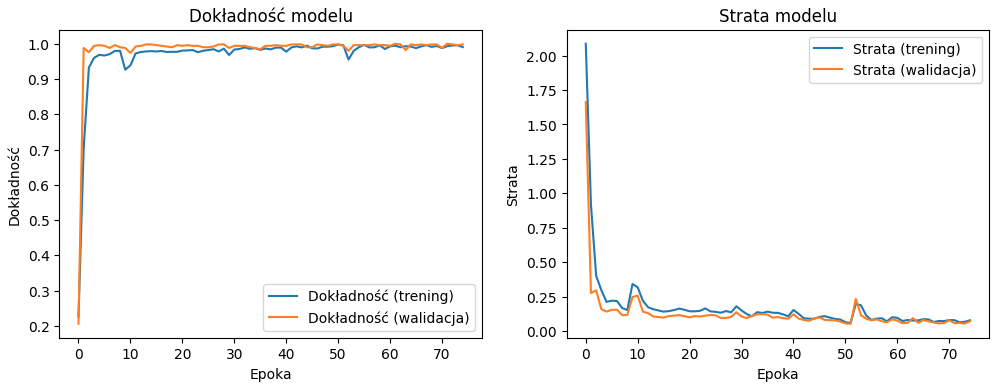
\includegraphics[width=14cm]{resources/tests/images/v4/multiple_edges_1_img.png}
	\caption{Dokładność i walidacja dla zmodyfikowanego modelu ze zmienną liczbą wierzchołków - Conv2D i Droput}
	\label{Fig:tests-var-1a}
\end{figure}
\FloatBarrier

Wydaje się, że model osiągnął pewną stabilność na niskim poziomie, co może pozytywnie świadczyć o jego zdolności generalizacji na nowe dane.

\begin{figure}[ht]
	\centering
	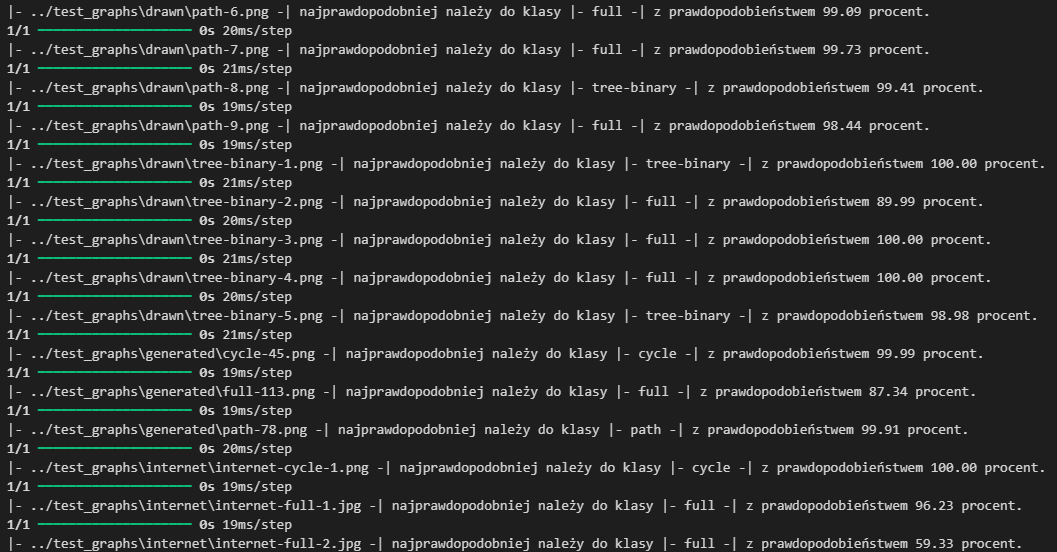
\includegraphics[width=14cm]{resources/tests/images/v4/multiple_edges_1_txt.png}
	\caption{Klasyfikacja obrazów zewnętrznych dla zmodyfikowanego modelu ze zmienną liczbą wierzchołków - Conv2D i Droput}
	\label{Fig:tests-var-1b}
\end{figure}
\FloatBarrier

\begin{figure}[ht]
	\centering
	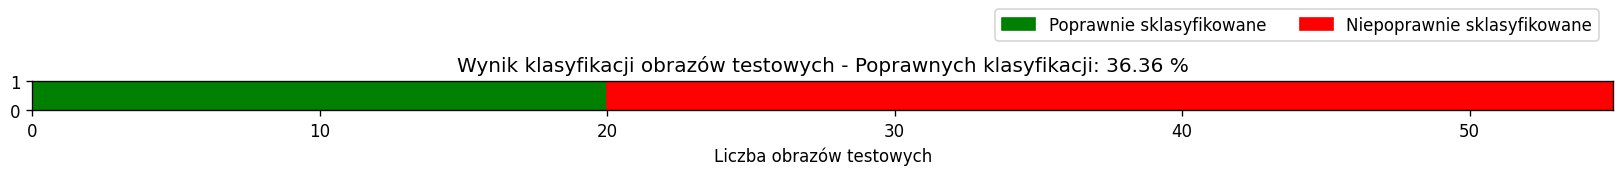
\includegraphics[width=14cm]{resources/tests/images/v4/multiple_edges_1_bar.png}
	\caption{Wizualizacja klasyfikacji obrazów zewnętrznych dla zmodyfikowanego modelu ze zmienną liczbą wierzchołków - Conv2D i Droput}
	\label{Fig:tests-var-0c}
\end{figure}
\FloatBarrier

Osiągnięta stabilizacja modelu i brak znaczących różnic między wartościami dokładności,
czy straty na zbiorach treningowych i wdalidacyjnych, nie przełożyła się w sposób rewolucyjny na osiągi modelu.
Model jednakże nie wypadł całkowicie źle - poprawnie sklasyfikował 36\% zewnętrznych grafów testowych,
co plasuje go w czołówce testowanych modeli pod kątem realnej dokładności.

\textbf{Zmodyfikowany model}

Do modelu wprowadzone zostały modyfikacje na wzór tych ze zmodyfikowanego modelu z walidacją krzyżową.
Przetestowany został wariant z włączonymi wszystkimi modyfikacjami na raz.

Podobnie jak dla zmodyfikowanego modelu z walidacją krzyżową, dokładność treningowa jest bardzo wysoka (prawie 100\%),
ale dokładność walidacyjna nie jest ustabilizowana. Jej wartości oscylują w przedziale od 0,2, aż do 0,9.
To sugeruje, że model nie generalizuje dobrze na nowych danych i może być nadmiernie dopasowany.

Wykresy straty prezentują się w podobny sposób jak i wykresy dokładności.
Strata treningowa jest bliska zeru, co mówi o świetnym zapamiętywaniu danych treningowych przez model, kosztem generalizacji na nowe dane.
Strata walidacji jednak jest niestabilna z bardzo wysokimi wartościami w niekórych epokach.

\begin{figure}[ht]
	\centering
	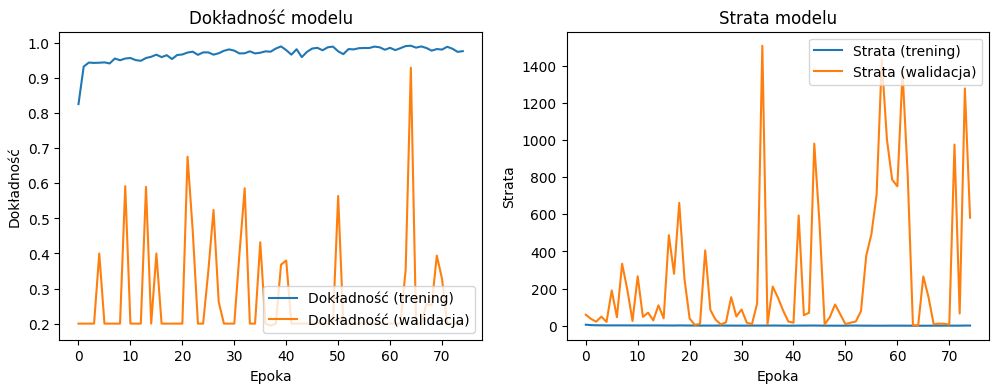
\includegraphics[width=14cm]{resources/tests/images/v4/multiple_edges_img.png}
	\caption{Dokładność i walidacja dla w pełni zmodyfikowanego modelu ze zmienną liczbą wierzchołków}
	\label{Fig:tests-var-2a}
\end{figure}
\FloatBarrier

Model wykazuje cechy modelu przeuczonego.
Są to bardzo wysoka dokładność i niemal zerowa strata na zbiorze treningowym
oraz bardzo niska dokładność i wysoka, ale niestabilna strata na zbiorze walidacyjnym.
Wniosek jaki można wyciągnąć jest taki, że model zapamiętał dane treningowe, ale nie nauczył się żadnych wzorców.

\begin{figure}[ht]
	\centering
	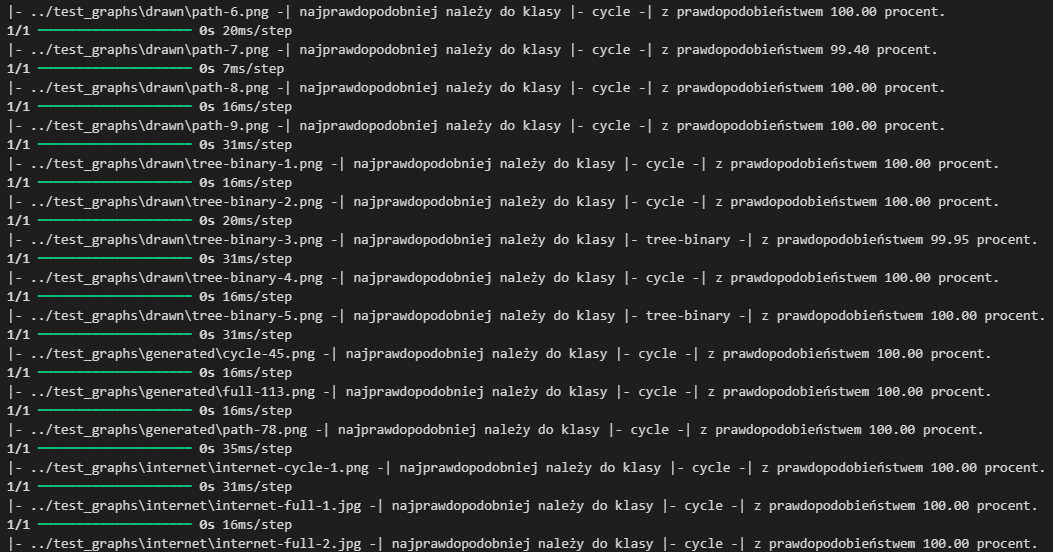
\includegraphics[width=14cm]{resources/tests/images/v4/multiple_edges_txt.png}
	\caption{Klasyfikacja obrazów zewnętrznych dla w pelni zmodyfikowanego modelu ze zmienną liczbą wierzchołków}
	\label{Fig:tests-var-2b}
\end{figure}
\FloatBarrier

\begin{figure}[ht]
	\centering
	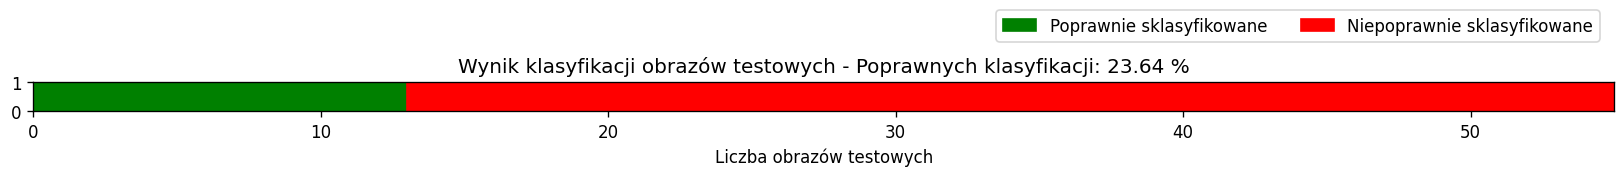
\includegraphics[width=14cm]{resources/tests/images/v4/multiple_edges_bar.png}
	\caption{Wizualizacja klasyfikacji obrazów zewnętrznych dla w pelni zmodyfikowanego modelu ze zmienną liczbą wierzchołków}
	\label{Fig:tests-var-2c}
\end{figure}
\FloatBarrier

Model poprawnie wskazał tylko około 24\% grafów, lecz analiza jego wskaźników mówi nam,
że jest to dzieło raczej przypadku, aniżeli poprawnego nauczenia się ogólnych wzorców danych.
Jego dokładność walidacyjna była bardzo niestabilna.

\section{Model ze zmienną liczbą wierzchołków i~walidacją krzyżową}
\subsubsection{Wersja podstawowa modelu ze zmienną liczbą wierzchołków i~walidacją krzyżową}

Model uczony na~grafach ze zmienną liczbą wierzchołków oraz zastosowaną walidacją krzyżową,
bardzo szybko osiąga poziom dokładności biski 100\%, bo już w~kilku pierwszych epokach.
Po około 10 epoce, dokonuje się stabilizacja, oscylująca między 95\%, a~100\%.
W przypadku tego modelu, fluktuacje dokładności są znikome, co wskazuje na~dobrą stabilność modelu.
Pojedyncze przypadku spadu dokładności, mogą być spowodowane bardziej skomplikowanymi
przypadkami w~zbiorze danych walidacyjnych.

Strata tego modelu gwałtownie spada na~początku procesu uczenia,
po czym stabilizuje się na~zadowalająco niskim poziomie - poniżej 20\%.
Skoki wskaźnika są bardziej zauważalne na~zbiorze walidacyjnym,
ale nie wydają się być regularne i~nie wpływają na~ogólny wynik.
Mogą być wynikiem, przeuczenia na~pojedynczych epokach lub~naturalną zmiennością walidacyjnego zbioru danych.

\begin{figure}[ht]
	\centering
	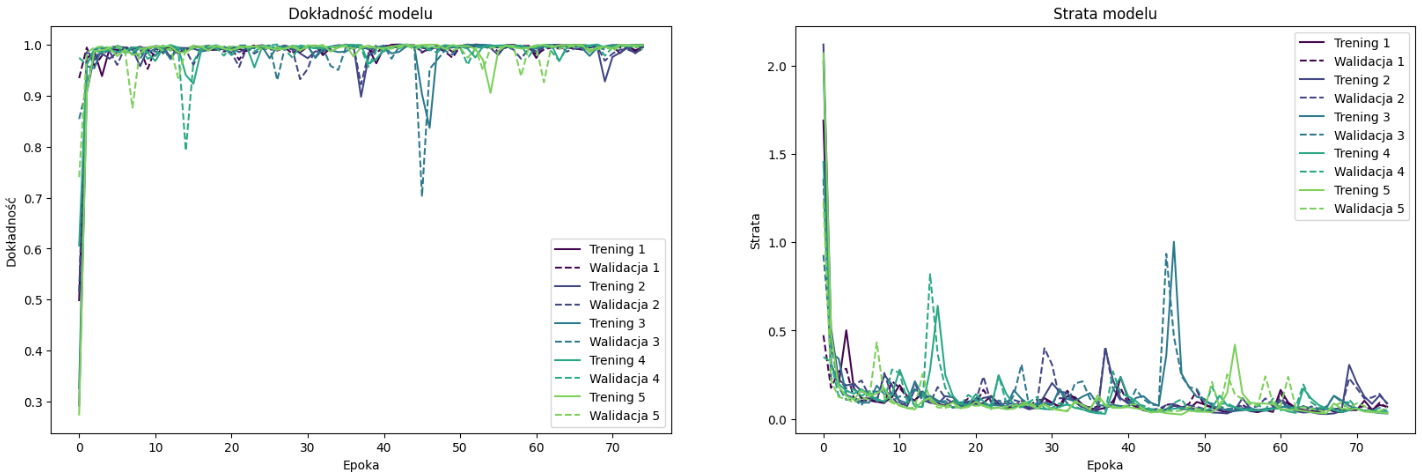
\includegraphics[width=15.5cm]{resources/tests/images/v3/multiple_edges_crossvalid_img.png}
	\caption{Dokładność i~walidacja dla modelu ze zmienną liczbą wierzchołków i~walidacją krzyżową}
	\label{Fig:tests-csvar-0a}
\end{figure}
\FloatBarrier

Model wydaje się dokładny na~zbiorze treningowym i~walidacyjnym,
co może skutkować polepszoną skutecznością w~klasyfikacji grafów.
Minimalne różnice pomiędzy dokładnością treningową a~walidacyjną wskazują na~dobrą zdolność generalizacji.
Z otrzymanych wyników, wydawałoby się, że model nie uległ przeuczeniu,
choć jest to~również możliwe, zważając na~bardzo wysokie wyniki dokładności. 

\begin{figure}[ht]
	\centering
	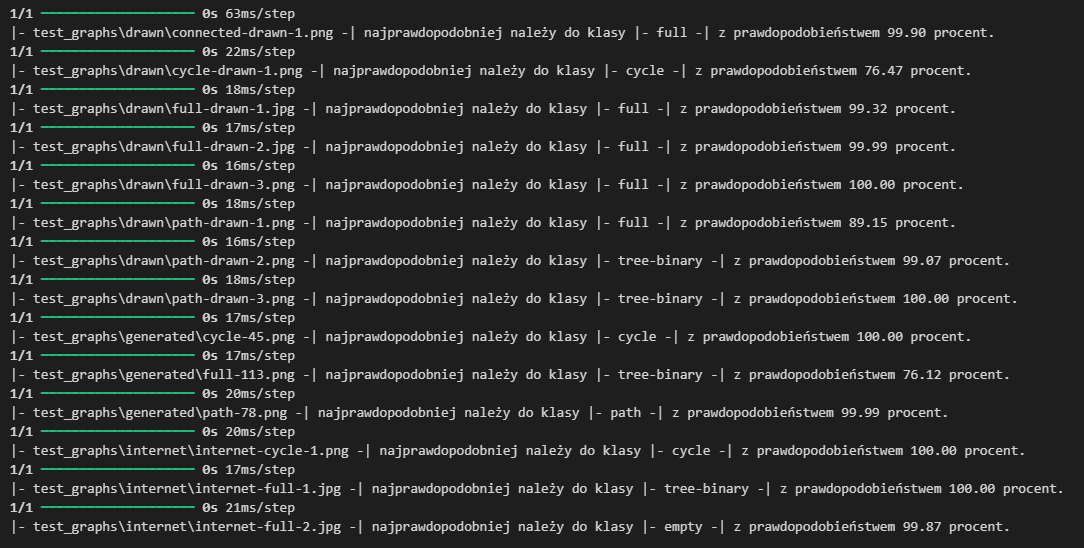
\includegraphics[width=15.5cm]{resources/tests/images/v3/multiple_edges_crossvalid_txt.png}
	\caption{Klasyfikacja obrazów zewnętrznych dla modelu ze zmienną liczbą wierzchołków i~walidacją krzyżową}
	\label{Fig:tests-csvar-0b}
\end{figure}
\FloatBarrier

\begin{figure}[ht]
	\centering
	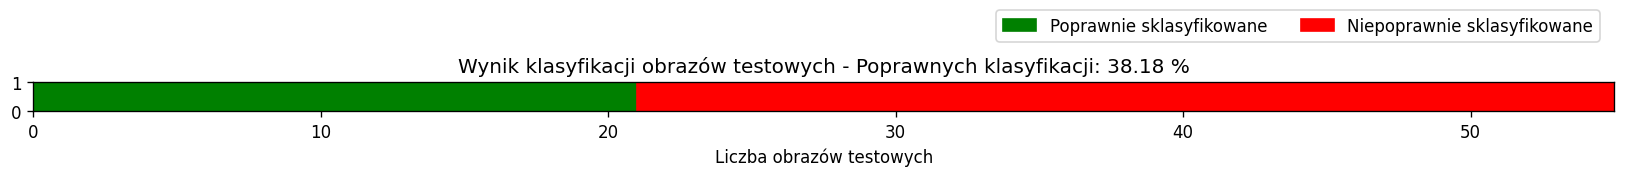
\includegraphics[width=15.5cm]{resources/tests/images/v3/multiple_edges_crossvalid_bar.png}
	\caption{Wizualizacja klasyfikacji obrazów zewnętrznych dla modelu ze zmienną liczbą wierzchołków i~walidacją krzyżową}
	\label{Fig:tests-csvar-0c}
\end{figure}
\FloatBarrier

Model poprawnie sklasyfikował aż 38\% testowanych danych zewnętrznych.
Jest to~zadowalający wynik, zważając na~trudności innych modeli w~poprawnym wskazywaniu klas sprawdzanych grafów.
Podejrzenia dotyczące przeuczenia modelu były więc bezpodstawne.
Model całkiem dobrze nauczył się żądanych wzorców.

\begin{figure}[ht]
	\centering
	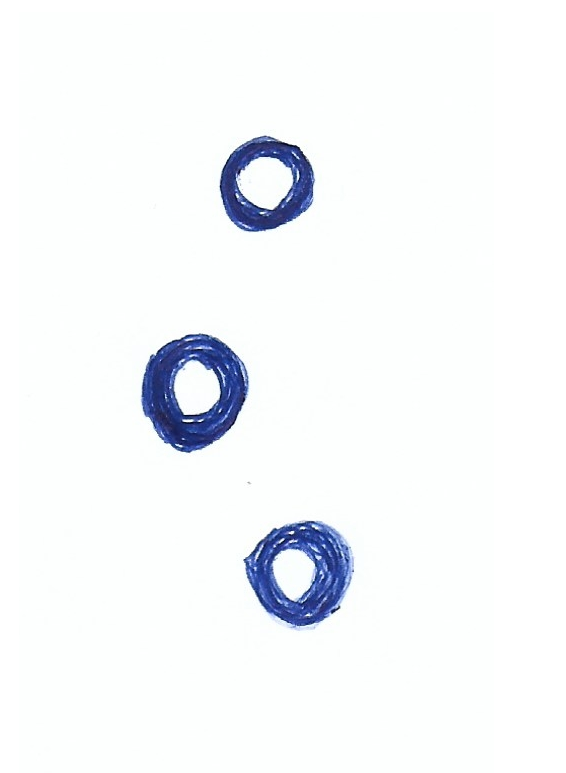
\includegraphics[height=4cm]{../graph_classification/test_graphs/drawn/empty-5.png}
	\caption{Klasyfikacja przykładowego grafu zewnętrznego przez model ze zmienną liczbą wierzchołków i~walidacją krzyżową.
		Przypisana klasa to~graf pełny z~100\% pewnością.}
	\label{Fig:tests-csvar-0d}
\end{figure}
\FloatBarrier

\subsubsection{Zmodyfikowany model ze zmienną liczbą wierzchołków i~walidacją krzyżową - Conv2D i~Dropout oraz spowolnienie uczenia}

Model stosuje zwiększone parametry filtrów dla warstw Conv2D, powiększony parametr Dropout z~0,2 do 0,5
oraz spowolnienie uczenia.

Dokładność osiąga poziom bliski 100\% na~zbiorze treningowym i~walidacyjnym w~bardzo szybkim tempie.
Po osiągnięciu tego pułapu, utrzymuje się na~nim do ostatniej epoki procesu nauczania modelu.
Jedyną anomalię można zaobserować około 55 epoki dla jednego z~przejść walidacji krzyżowej.
Spada ona gwałtownie do poziomu 23\% i~pozostaje w~takim stanie do końca nauki.

Strata prezentuje się podobnie jak dokładność.
Wartości utrzymują się na~dość niskich poziomach przez cały proces uczenia po początkowym spadku.
Około 55 epoki, dla jednego przejścia walidacji krzyżowej,
da się zaobserować nagły wzrost straty do około 2,5 jednostek, który stopniowo spada do około 1,8.

\begin{figure}[ht]
	\centering
	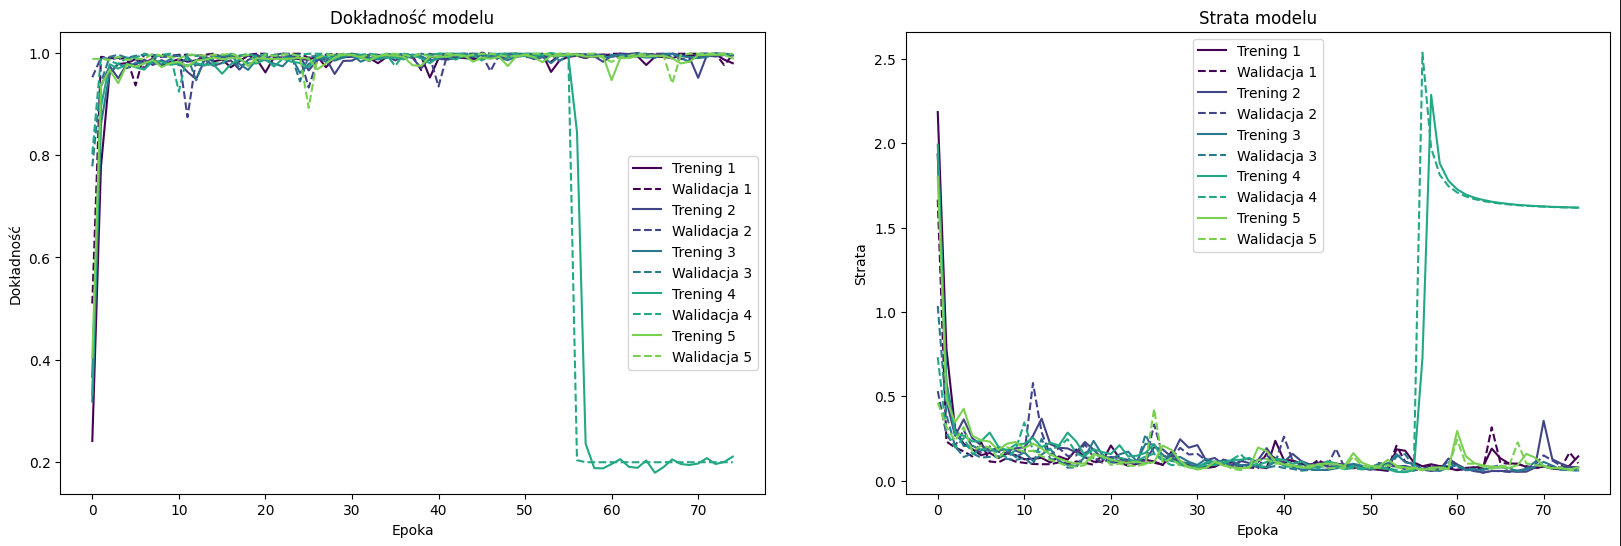
\includegraphics[width=15.5cm]{resources/tests/images/v4/multiple_edges_crossvalid_1_img.png}
	\caption{Dokładność i~walidacja dla zmodyfikowanego modelu ze zmienną liczbą wierzchołków i~walidacją krzyżową - Conv2D i~Droput}
	\label{Fig:tests-csvar-1a}
\end{figure}
\FloatBarrier

W przypadku pojedynczej anomalii jaką da się zaobserować na~krzywych dokładności oraz straty,
można wnioskować, że dla jednego przejścia walidacji krzyżowej, a~konkretnie czwartego, wystąpił pewien problem z~uczeniem modelu.
Mogła to~być zmiana wartości współczynnika uczenia się lub~inna zmiana w~procesie treningu.
Różnice pomiędzy wartościami dla danych treningowych oraz waldacyjnych są znikome - nawet w~przypadku odstającym wartościami od reszty.
Ogólnie, model osiągnął bardzo dobre wyniki, co sugeruje, że proces nauczania przebiegł pomyślnie.

\begin{figure}[ht]
	\centering
	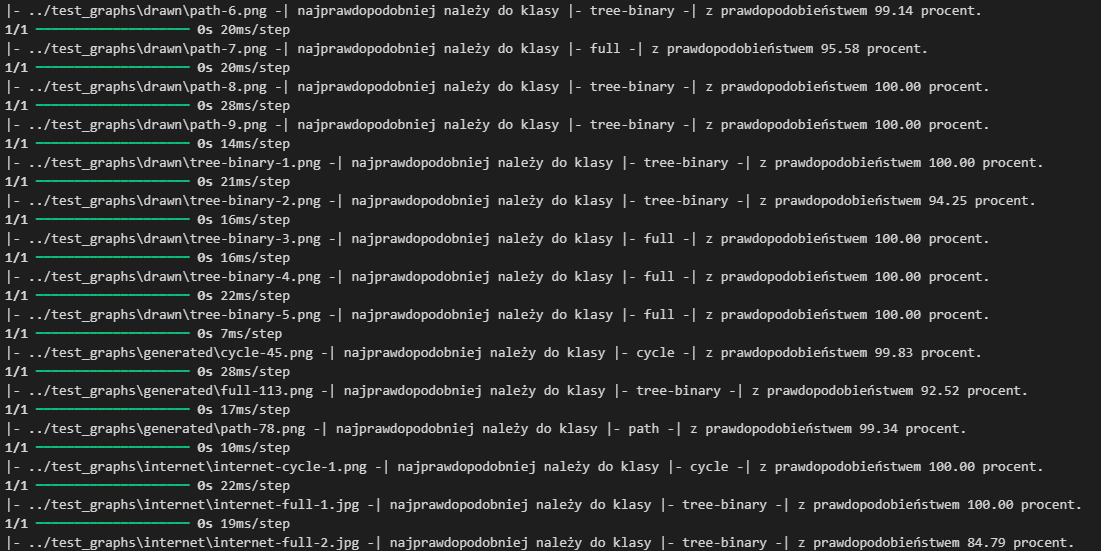
\includegraphics[width=15.5cm]{resources/tests/images/v4/multiple_edges_crossvalid_1_txt.png}
	\caption{Klasyfikacja obrazów zewnętrznych dla zmodyfikowanego modelu ze zmienną liczbą wierzchołków i~walidacją krzyżową - Conv2D i~Droput}
	\label{Fig:tests-csvar-1b}
\end{figure}
\FloatBarrier

\begin{figure}[ht]
	\centering
	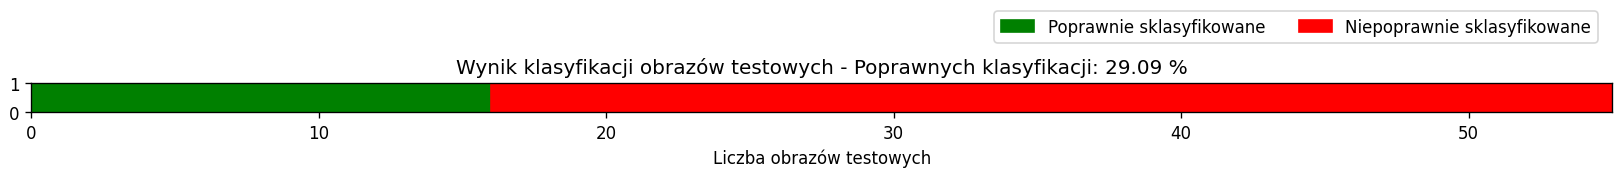
\includegraphics[width=15.5cm]{resources/tests/images/v4/multiple_edges_crossvalid_1_bar.png}
	\caption{Wizualizacja klasyfikacji obrazów zewnętrznych dla zmodyfikowanego modelu ze zmienną liczbą wierzchołków i~walidacją krzyżową - Conv2D i~Droput}
	\label{Fig:tests-csvar-1c}
\end{figure}
\FloatBarrier

Poprawna klasyfikacja 29\% grafów jest w~pewnym sensie rozczarowującym wynikiem,
zważajac na~wysokie wartości dokładności, nawet na~zbiorach walidacyjnych
oraz całkiem wysoki wynik modelu bez modyfikacji.
Wnioskować można, że spowolnienie uczenia i~zwiększenie liczby filtrów w~warstwach Conv2D oraz zwiększenie parametru dropout,
nie przyniosło oczekiwanych skutków.

\begin{figure}[ht]
	\centering
	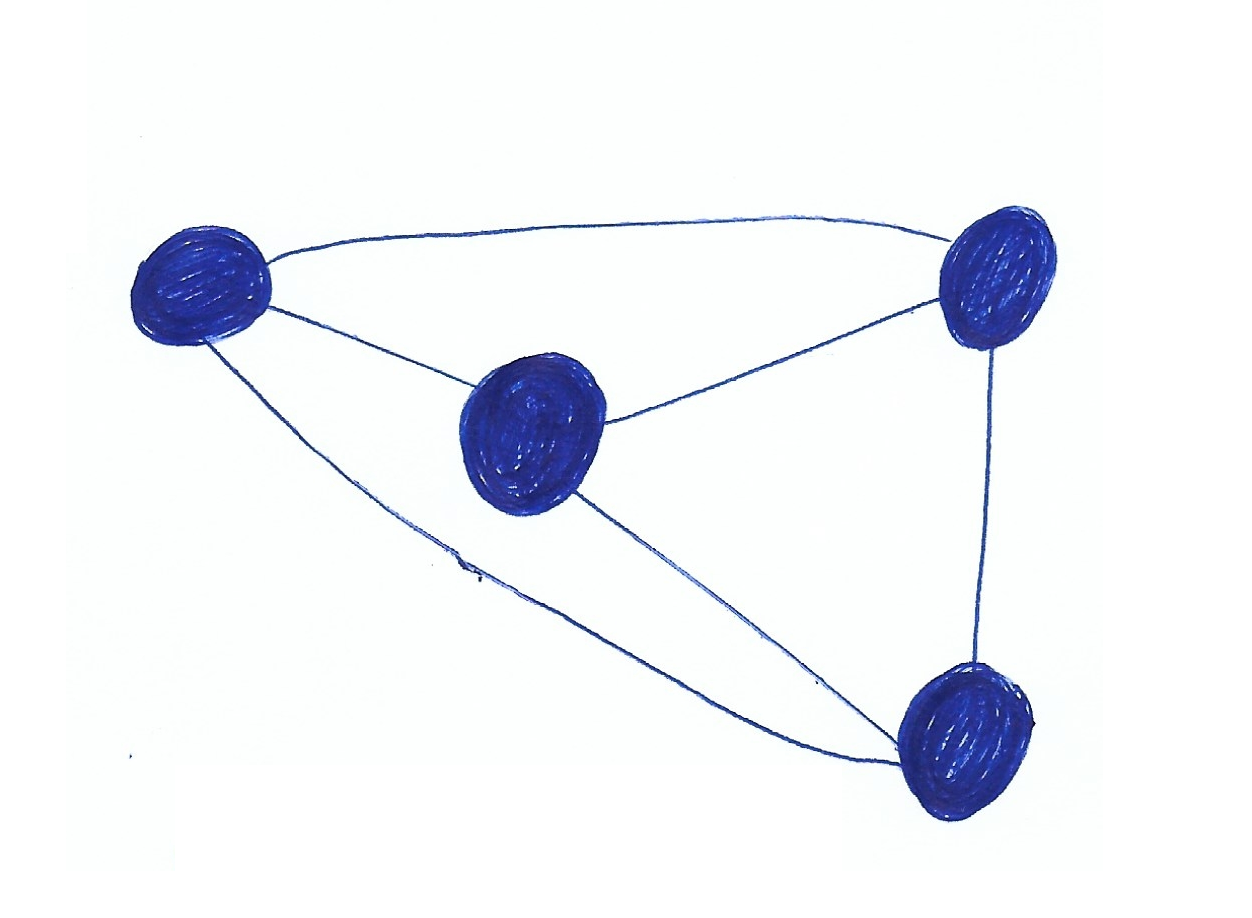
\includegraphics[height=4cm]{../graph_classification/test_graphs/drawn/full-10.png}
	\caption{Klasyfikacja przykładowego grafu zewnętrznego przez
		zmodyfikowany model ze zmienną liczbą wierzchołków i~walidacją krzyżową - Conv2D i~Dropout oraz spowolnienie uczenia.
		Przypisana klasa to~drzewo binarne z~99,95\% pewnością.}
	\label{Fig:tests-cv-1d}
\end{figure}
\FloatBarrier

\subsubsection{Zmodyfikowany model ze zmienną liczbą wierzchołków i~walidacją krzyżową - modyfikacje połączone}

Do modelu wprowadzone zostały wszystkie modyfikacje wymienione w~rozdziale z~modelem z~walidacją krzyżową,
czyli zwiększenie liczby filtrów w~warstwach, normalizacja wsadowa, augmentacja danych oraz zmniejszenie szybkości uczenia.

Model dość szybko osiąga wysoką dokładność na~zbiorze treningowym - stabilizuje się około 90-95\%.
Podobnie jak i~w innych modelach z~zastosowanymi wszystkimi modyfikacjami,
dokładność na~zbiorze walidacyjnym jest niestabilna.
Można zaobserować duże wahania pomiędzy kolejnymi epokami procesu uczenia.
Sugeruje to~trudności z~uczeniem się wzorców.

Model szybko zmniejsza stratę treningową i~pozostaje ona na~bardzo niskim poziomie przez cały proces uczenia.
Wskazuje to~na~sprawność w~uczeniu się na~danych treningowych.
Wykresy strat przedstawiają się w~nietypowej formie.
Dla początkowych i~końcowych epok, straty walidacji niewiele się wahają,
a wręcz przeciwnie sytuacja wygląda dla epok od około dziesiątej do dwudziestej.
Model ma więc trudności z~radzeniem sobie z~danymi, które są dla niego nowe.

\begin{figure}[ht]
	\centering
	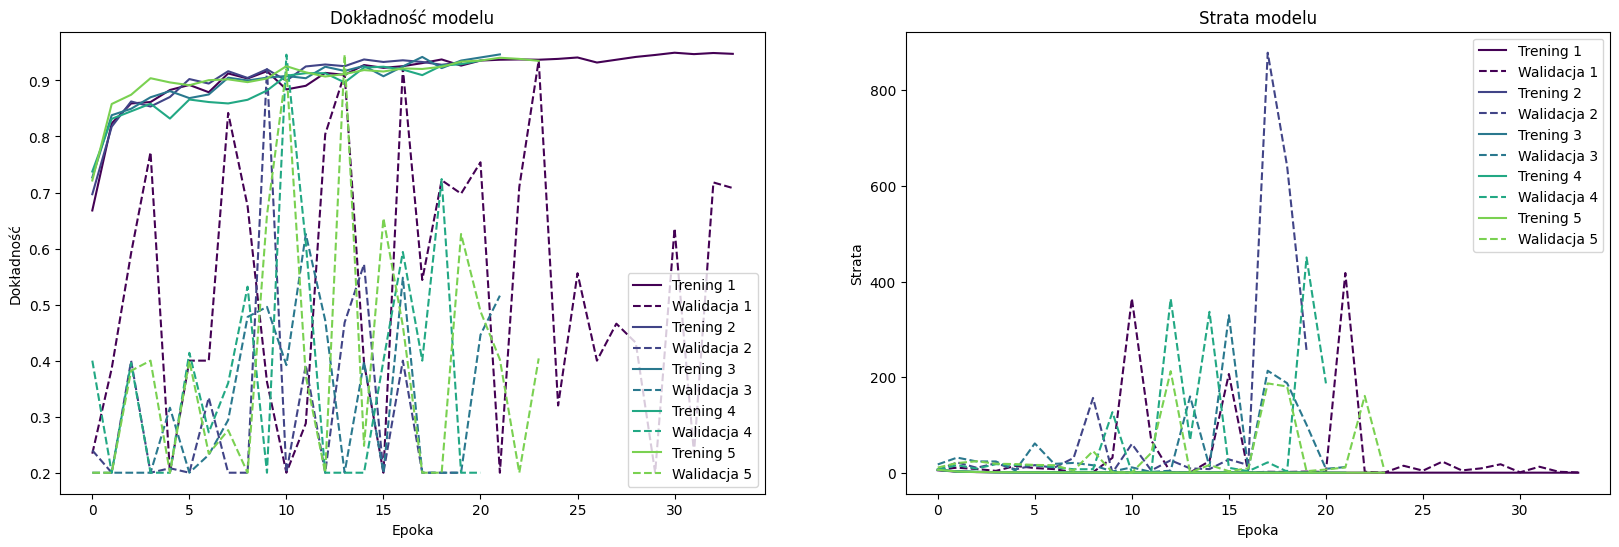
\includegraphics[width=15.5cm]{resources/tests/images/v4/multiple_edges_crossvalid_img.png}
	\caption{Dokładność i~walidacja dla w~pełni zmodyfikowanego modelu ze zmienną liczbą wierzchołków i~walidacją krzyżową}
	\label{Fig:tests-csvar-2a}
\end{figure}
\FloatBarrier

Model osiąga bardzo wysokie wyniki na~zbiorze treningowym,
ale ma problemy z~generalizacją na~zbiorze walidacyjnym.
Wskazuje to~na~przeuczenie modelu i~brak uczenia się wzorców ogólnych.

\begin{figure}[ht]
	\centering
	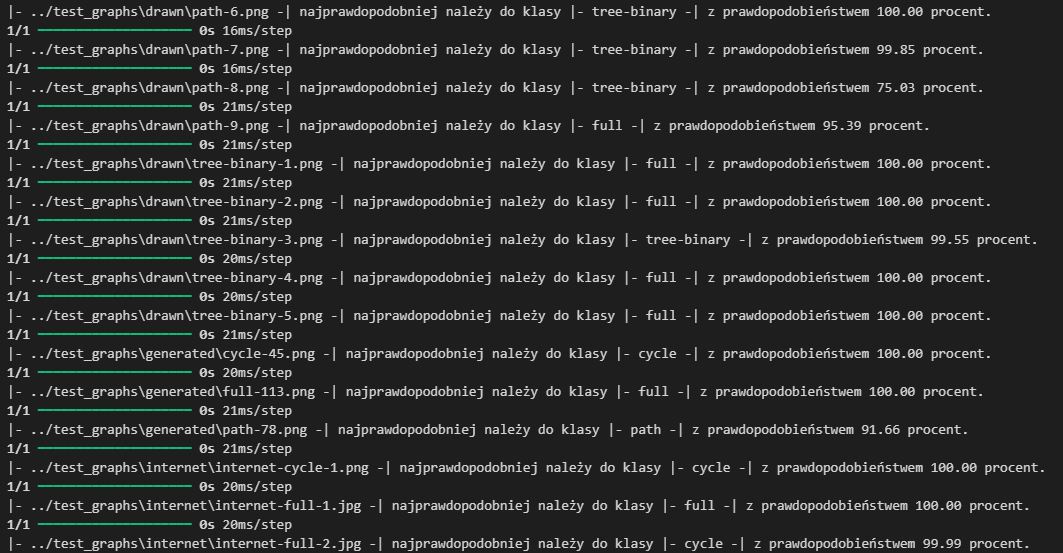
\includegraphics[width=15.5cm]{resources/tests/images/v4/multiple_edges_crossvalid_txt.png}
	\caption{Klasyfikacja obrazów zewnętrznych dla w~pełni zmodyfikowanego modelu ze zmienną liczbą wierzchołków i~walidacją krzyżową}
	\label{Fig:tests-csvar-2b}
\end{figure}
\FloatBarrier

\begin{figure}[ht]
	\centering
	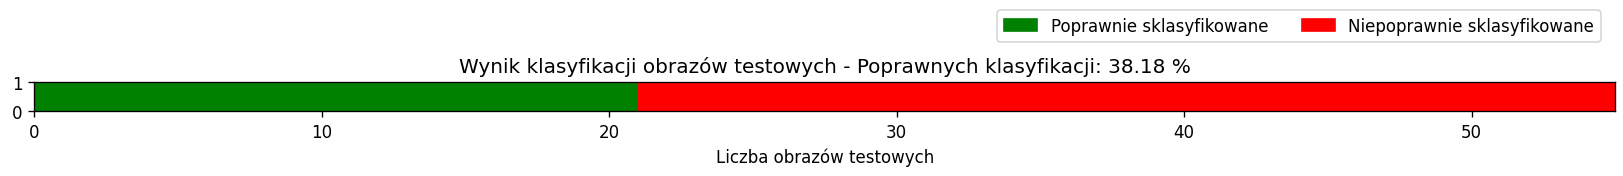
\includegraphics[width=15.5cm]{resources/tests/images/v4/multiple_edges_crossvalid_bar.png}
	\caption{Wizualizacja klasyfikacji obrazów zewnętrznych dla w~pełni zmodyfikowanego modelu ze zmienną liczbą wierzchołków i~walidacją krzyżową}
	\label{Fig:tests-csvar-2c}
\end{figure}
\FloatBarrier

Model ocenił poprawnie około 38\% klas grafów zewnętrznych, co nie jest złym wynikiem.
W przypadku modeli z~walidacją krzyżową, zastosowanie wszystkich przygotowanych modyfikacji modelu,
nie do końca spełniło swoje złożenia, ale również nie pogorszyło wyniku.

\begin{figure}[ht]
	\centering
	\includegraphics[height=4cm]{../graph_classification/test_graphs/drawn/cycle-2.png}
	\caption{Klasyfikacja przykładowego grafu zewnętrznego przez zmodyfikowany model
		ze zmienną liczbą wierzchołków i~walidacją krzyżową - modyfikacje połączone.
		Przypisana klasa to~cykl z~100\% pewnością.}
	\label{Fig:tests-cv-2d}
\end{figure}
\FloatBarrier

\section{Modyfikacje modelu o~najlepszej dokładności realnej}
W wyniku testów wyłoniony został model o najlepszej dokładności realnej, tj.
dokładności klasyfikacji zewnętrznych grafów testowych.
Model ten okazał się jednym z najbardziej podstawowych z przygotowanych,
bo jest to podstawowy model uczony na grafach sześciowierzchołkowych.
W ramach eksperymentu, zastosowano dla niego modyfikacje,
które pomogły zwiększyć realną dokładność modelu.
Modyfikacje te zostały wprowadzone i przetestowane w podrozdziale z testami modeli
z walidacją krzyżową.
Jedyną zmianą z zaproponowanych, która przynosi realne korzyści,
jest zwiększenie liczby filtrów w warstwach sieci neuronowej, kolejno 32, 64 oraz 128 dla Conv2D,
oraz zastosowanie zwiększonego parametru dropout - 0,5.

\textbf{Zmodyfikowany model podstawowy uczony na grafach sześciowierzchołkowych}

Model osiąga poprawne wyniki, lecz po około 55 epoce procesu nauczania,
dokładność gwałtownie spada, aż do wartości około 23\%.

Ta sama sytuacja dotyczy straty, która to gwałtownie wzrasta około 60 epoki,
z około 0,25, do aż 1,75.

\begin{figure}[ht]
	\centering
	\includegraphics[height=5.5cm]{resources/tests/images/v4/base6_1_img.png}
	\caption{Wyniki testów dla zmodyfikowanego modelu podstawowego, liczba wierzchołków = 6}
	\label{Fig:tests-base-5a}
\end{figure}
\FloatBarrier

% \begin{figure}[ht]
% 	\centering
% 	\includegraphics[width=14cm]{resources/tests/images/v4/base6_1_txt.png}
% 	\caption{Klasyfikacja obrazów zewnętrznych dla zmodyfikowanego modelu podstawowego, liczba wierzchołków = 6}
% 	\label{Fig:tests-base-5b}
% \end{figure}
% \FloatBarrier

% \begin{figure}[ht]
% 	\centering
% 	\includegraphics[width=14cm]{resources/tests/images/v4/base6_1_bar.png}
% 	\caption{Wizualizacja klasyfikacji obrazów zewnętrznych dla zmodyfikowanego modelu podstawowego, liczba wierzchołków = 6}
% 	\label{Fig:tests-base-5c}
% \end{figure}
% \FloatBarrier

\textbf{Zmodyfikowany poprawiony model podstawowy uczony na grafach sześciowierzchołkowych}

Wyniki uzyskane z procesu nauki poprzeniego modelu sugerują zmniejszenie liczby epok do około 55.
Taka modyfikacja została zastosowana, a test przeprowadzono ponownie.

% -- TO DO -- % Dokładność

% -- TO DO -- % Strata

\begin{figure}[ht]
	\centering
	\includegraphics[height=5.5cm]{resources/tests/images/v4/base6_1_1_img.png}
	\caption{Wyniki testów dla poprawionego zmodyfikowanego modelu podstawowego, liczba wierzchołków = 6}
	\label{Fig:tests-base-6a}
\end{figure}
\FloatBarrier

% -- TO DO -- % Opis ogólny

\begin{figure}[ht]
	\centering
	\includegraphics[width=14cm]{resources/tests/images/v4/base6_1_1_txt.png}
	\caption{Klasyfikacja obrazów zewnętrznych dla poprawionego zmodyfikowanego modelu podstawowego, liczba wierzchołków = 6}
	\label{Fig:tests-base-6b}
\end{figure}
\FloatBarrier

\begin{figure}[ht]
	\centering
	\includegraphics[width=14cm]{resources/tests/images/v4/base6_1_1_bar.png}
	\caption{Wizualizacja klasyfikacji obrazów zewnętrznych dla poprawionego zmodyfikowanego modelu podstawowego, liczba wierzchołków = 6}
	\label{Fig:tests-base-6c}
\end{figure}
\FloatBarrier

% -- TO DO -- % Opis klasyfikacji